\documentclass[11pt,letterpaper,twoside]{article}
\usepackage[tmargin=1in,bmargin=1in,lmargin=1in,rmargin=1in]{geometry}
\usepackage{../style/packages}
\usepackage{../style/commands}
\setbool{notesonly}{false}

% -------------------
% Content
% -------------------
\begin{document}

% Cover Photo
% !TEX root = ../main/aws_topandarith.tex

\thispagestyle{empty}
\newgeometry{
	top=0cm, 
	bottom=0cm, 
	left=0cm, 
	right=0cm
}


\tikz[remember picture,overlay] \node[opacity=1,inner sep=0pt] at (current page.center){
\includegraphics[width=\paperwidth,height=\paperheight]{../cover/swc_poster.jpg}};

\phantom{x} % To image is placed.

% Reset Page Style
\newgeometry{
	top= 1in, 
	bottom= 1in, 
	left= 1in, 
	right= 1in
}
\newpage

% Cover
% !TEX root = ../main/aws_topandarith.tex

\thispagestyle{empty}
\begin{flushright}
\begin{tabular}{ll}
\raisebox{-.5\height}{
\includegraphics[scale=0.055]{../cover/arizona_seal.png}} & {\color{ArzBlue} \Huge University of Arizona} \\
\end{tabular}
\end{flushright}
\vspace{2in}

{%
\color{ArzRed} \Huge \noindent Arizona Winter School 2019 \\[0.2cm] \Huge \color{ArzRed} Topology and Arithmetic \\[0.2cm] \color{ArzBlue}
\rule{0.70\textwidth}{0.05cm} \vspace{0.1cm}
}

{\color{ArzBlue} \large \noindent Notes By: Caleb McWhorter }

\vfill
\begin{center} {\color{ArzBlue}\huge March 2019} \end{center}
\newpage

% TOC
\thispagestyle{blank}
\tableofcontents
\newpage

% -------------------
% Lectures
% -------------------

% Lecture Notes
\thispagestyle{empty}
\part{Talk Notes} 
    \newpage 
	\setcounter{page}{1}

% Hopkins
% !TEX root = ../../../main/aws_topandarith.tex
\newpage
\section{Name: Lecture Title}
\subsection{Lecture 1}
\subsubsection{Lecture Name}

We start with the famous theorem of Kronecker-Weber Theorem.

\begin{thm}
If $K/\Q$ is an abelian Galois extension, then $K= \Q(\zeta_n)$ for some $n$, where $\zeta_n$ is a (primitive) $n$th root of unity. 
\end{thm}

Kronecker's famous JugendTraub. Want to construct? Using the roots of unity. to make abelian Galois extensions. 





Lubin-Tate: Get Galois extensions using formal groups. Formal group law over $R$. $F(x,y)= x\fplus y= x + y + \cdots$

$x\fplus 0 = 0\fplus x= x$
$x\fplus y= y \fplus x$
$(x \fplus y) \fplus z = x \fplus (y \fplus z)$

Lie variety over $R$
Objects $\A^n$, $n= 0,1,\ldots$
maps $\A^n \to \A^1$, $f(x_1,\ldots,x_n) \in R[x_1,\ldots,x_n]$
$\A^n= A^n \to \prod \A^1$ 


Question: How many formal group laws are there? How to construct formal group laws?

\begin{thm}[Lazard]
$R \mapsto$ formal group laws over $R$, ring($L,R$), $L= \Z[x_1,x_2,\ldots]$.
\end{thm}

Isomorphism $F \ma{g} G$
$g(x)$
$g(x \fplus y)= g(x) \fplus g(y)$

Universal isomorphism over $L[s_1,s_2,\ldots]$



Algebraic Topology

Cohomology theories $E$ with Chern classes in complex line bunles,
$V /X \to c_i(X) \in E^{2n}(X)$
$c_n(V\C)_N= \sum_{i+j=n} c_i(Y) c_j(W)$

Not true in general $c_1(L_1 \otimes L_2)= c_1(L_1)$


\begin{thm}[Quillen]
For general, $E$, there exists a formal group law $F$
$c_1(L_1 \otimes L_2)= F(c_1(L_1),c_1(L_2))= c_1(L_1) \fplus c_1(L_2)$
\end{thm}

$H^s(\m_{FG}, \omega^*) \Rightarrow \pi_{2t-s}S^0= \lim_{n \to \infty} \pi_{2t-s+n} S^n$
$\omega= \lie F^*$

% Give picture


\begin{ex}
$G_n$ $x+y$
$G_m$ $x+y-xy= 1-(1-x)(1-y)$

Are these isomorphic?

$g(x)= 1 - e^{-x}$
$g(x+y) \stackrel{=}{\text{maybe}}= g(x)g(x) - g(x)g(y)$
over $\Q$-algebra
So isomorphic over rationals.

Are they isomorphic over $\F_p$? Are there even homomorphisms between them?
Suppose $g: G_n \to G_m$ is one such
$g(x+\cdots+x)= 1-(1- g(x))^p$
$0= g(0)= g(x)^4= g^0(x^p)$ so that $g=0$ so no homomorphisms from additive group to multiplicative group. 
\end{ex}


Height: 

$R=k$ field of char $p>0$
$f: G_1 \to G_2$
Then there exists unique $g(x)$, $g'(0) \neq 0$, $y= p^a$
$f(x)= g(x^q)$
$a$ is the height of $f$.
Height of a formal group is by definition the height of mult by $p$
height $G_n= \infty$
height $G_m= 1$

\begin{thm}[Dieudonne]
$k$ perfect algebraically closed, any two formal groups of the same height are isomorphic. 
\end{thm}


Lubin-Tate deformation spaces
$\Gamma$, $k$ field char $p>0$, $B$ complete local $\m$-maximal local

A deformation of $\Gamma$ to $B$ 
$B \ma{r} B/\m \stackrel{i}{\leftarrow} k$

$(G,i,f)$, $G \ma{f} i^*\Gamma$
Deform$_\Gamma(B) \leftarrow$ groupoid

\begin{thm}[L-T]
$n=$ height of $\Gamma$
$\pi_0$ Deform$_\Gamma(B)= \m^{n-1}$
\end{thm}

We want to understand this set $\m^{n-1}$ mod by automorphisms of $\Gamma$.


$G_\text{univ}$ universal deformation 
$W[[u_1,\ldots,u_{n-1}]]$
$W$ witt vectors of $k$
Universal deformation


$E_0= W[[u_1-u_{n-1}]]$
$E_*= W[[U_1-u_{n-1}]][u,u^{-1}]$, $|u|= -2$

Aut $\Gamma= S_n$, acts on $E_*$
$UE_0= E_{-2}$ sections of Lie $G$
interested in $H^*(S_n; E_0)$, not the symmetric group
$H^*(S_n; E_{2n})$


Question: Can one write down explicitly the action of $\Aut \Gamma$ on $W[[u_1-u_{n-1}]]$.

Question: What is $\pic$(Lubin tate) $=H^1(\Aut \Gamma; E_0^*)$, conjectured answer enlists known $n=2$, $p>5$


Observation: $n=2$, $H^*(S_n; W) \ma{\sim} H^*(S_n;E_0)$
$p>3$ Shimomura
$p \leq 3$ Beaudiy, Bobkova, Behrens, Wenn, \dots
True for $n>2$?
















% !TEX root = ../../../main/aws_topandarith.tex
\newpage
\subsection{Lecture 2}

Ex: $G_m$,
$x+y-xy= 1 - (1-x)(1-y)$
over $\Z_p$
$\Aut G_m= \Z_p^\times$
$\lambda \in \Z_p^\times$
$x \mapsto 1 - (1-x)^\lambda$

Lubin-Tate ring $\Z_p$
$\Aut G_m$ acts trivially.

$E_0= W[[u_1,\ldots,u_{n-1}]]$
$E_*= W[[u\cdots u_{n+1}[u^{\pm 1}]$, $|u|= -2$

$\Z_p[u^{1/2}]$
$\lambda \in \Aut(G_m)= \Z_p^\times$
How does $\lambda$ act on $u$?

$u^{-1}$ is an invariant differential on $G_m$
$u^{-1}$ is $dx+ \cdots= (1-x)\;dx$

$1-(1-x)^\lambda= \lambda x + \text{hot}$
$u^{-1} \mapsto \lambda u^{-1}$. 

$H^*(\Z_p^\times: \Z_p[u^{\pm 1}])$, $p>2$
$\lambda^{-1} \in \Z_p^\times$
$\lambda^{-1}$ generates $\Z_p^\times$ map 
$(\lambda^{-1})^{p-1} \neq 1 \mod p^2$

$H^1(\Z_p^\times : u^n \Z_p)= \Z_p/(\lambda^n-1)$
$n \neq 0$

Makes sense for $\lambda \mapsto \lambda^n$
Replace by $\Hom(\Z_p^\times,\Z_p^\times)$


$n=2$ 
$\Gamma$ is formal group over $k$ of height 2
$H^*(\Aut \Gamma; W[[u_1]])=?$

It turns out, $p>3$
$\Lambda[x_1,x_3]=H^*(\Aut \Gamma; W) \ma{x} H^*(\Aut \Gamma; W[[u_1]])$


Dieudonne modules

$k$ perfect field
$W$ ring of Witt vectors of $k$
$k$ acts on $u$, $u(x)= x^p$
$W$ acts on $u$

Diuedonne-module:
$M$ free $W$-module of finite rank
$F: u^*M \to M$
$F(am)= a^u F(m)$ for a$a \in W$,

$V: M \to u^*M$
$V(a^um)= aUM$,
$FU=UF=p$

Formal groups over $k$ $\leftrightarrow$ diedonne modules

height $\leftrightarrow$ $\dim_W M$
dim $\leftrightarrow \dim_k M/VM$



Ex: $M$ basis $\gamma, U\gamma$
$F\gamma= V \gamma$

This $M$ $\leftrightarrow$ height 2 formal group over $k$


$n \neq $

$\{\gamma, V \gamma, \ldots, V^{n-1} \gamma\}$
$F\gamma= V^{b-1} \gamma$

$\Aut \Gamma$, ht 2
$\gamma \to a \gamma + b V \gamma$
$V\gamma \to a^{\phi^{-1}} V \gamma + b^{\phi^{-1}} V^2 \gamma = a^{\phi^{-1}} V \gamma + p b^{\phi^{-1}} \gamma$

$F\gamma \to a^{\phi} V \gamma + p b^\phi \gamma$
$a,b \in W\F_{p^2}$

$F\gamma = V\gamma$
$p \gamma = VF\gamma= V^2 \gamma$

$\Aut(\Gamma)= \{ \two{a}{pb^{\phi^{-1}}}{b}{a^{\phi^{-1}}} \colon a,b \in W\F_{p^2}\}$. 


Tapis de Cartier
	\[
	\begin{tikzcd}
	M \arrow[dotted]{r}{T} \arrow{d} & W \arrow{d} \\
	M/VM \arrow{r}{\sim} & k
	\end{tikzcd}
	\]
lifts of $\Gamma$ to $W$. 


Dotted map $W$-linear specialization $\gamma \to 1$?

Bottom map $\gamma \mapsto 1$

$U_1(T)= T(V\gamma)$
$W[[u_1]]$

$\gamma \ma{y} a \gamma + bV \gamma$
$V \gamma \to a^{\phi^{-1}} V \gamma + p b^{\phi^{-1}} \gamma$
$y(u_1)= (a^{\phi^{-1}} u_1 + pb^{\phi^{-1}})/(bu_1+a)$



Crystalline Approximation

$M \to E_{-2}= uW[[u_1 \cdots u_{n-1}]]$

$\gamma \to u$
$V \gamma \to uu_1$
$\vdots$
$V^{n-1}\gamma \to uu_{n-1}$
$\Aut \Gamma$ equivalent. 

$G$
$k \leftarrow W \rightarrow u \otimes W$ 
$G \cong O_n$

$\Gamma$

$f(\gamma) = \log_G(x)= x+ \cdots + u \otimes w[[x]]$
$f^{-1}(f(x)+f(y))= x \fplus y$


Ex: $\log_{G_m}(x)= \sum x^n/n$

$T: M \to W$
$f(x)= \sum T(F^n \gamma) x^{p^n}/p^n$
is the log of a formal $?$ over $W$


Ex: $G= G_m$
$M= ?\{\gamma\}$
$F\gamma= \gamma$

$\log = \sum x^{p^n}/p^n$

Ex: ht$=2$ 
$T(\gamma)=1$
$T(v\gamma)=0$
$f(y)= \sum x^{p^{2n}}/p^n= l(x)$

$W[[w_1]]$
$T(\gamma)=1$
$T(V\gamma)=W_1$

$f(x)= l(x)+ w_1/p l(x^p)$
$f^{-1}(f(y)+f(y))$ does not have coefficients in $?[[w_1]]$

It does have coefficient in the divided power completion $w<<w_1>>$. 







































% !TEX root = ../../../main/aws_topandarith.tex
\newpage
\section{Name: Lecture Title}
\subsection{Lecture 1}
\subsubsection{Lecture Name}

Last time: $l(x)= \sum x^{p^{2n}}/p^n$
is the log at a formal group over $W$
$l^{-1}(l(x)+l(y)) \in W[[x,y]]$

$f(x)= l(x) + w_1/p l(x^p)$

not the log of a formal grouo


$W[[u_1\cdots u_{n-1}]]$
acted on by $\phi$, $\phi(u_i)= u_i^p$
$\phi$ Frob on $W$

$f(x)= x + u_1/p + f^\phi(x^p) + \cdots + u_{n-1}/p f^{\phi^{n-1}}(x^{p^n}) + 1/p f^{\phi^n}(x^{p^n})$

$n=2$
$f(x)= \sum m_k x^{p^k}$
$m_0=1$
$m_1= u_1/p$
$m_2= 1/p+ u_1^{1+p}/p^2$


$p \in I \unlhd A \subset L$
$\phi: L \to L$
$\phi: A \to A$
$\phi(x) \epsilon x^p \mod I$

$s_1,\ldots, \in L$
$\forall \phi^i(s_j) \cdot I \subseteq A$. 


Nazewinkel

$f(x)= x + s_1 f^\phi(x^p) + \cdots + s_n f^{\phi^n}(x^{p})$

Then $f^{-1}(f(x) + f(y)) \in A[[x,y]]$

$l(x)= \sum x^{p^m}/p^n$
$l(x)= x + 1/p l(x^{p^2})$

$f(x)= l(x) + w_1/p l(x^p)$

If we took $\phi(w_1)=0$
$f(x)= x + w_1/p f^\phi(x^p) + 1/p f^{\phi^2}(x^{p^2})$

$I=(p)$
$\phi(w_1)=0$, need $w_1^p \equiv 0(p)= w_1^p/p = w^{cn}$

$\phi(w^{(1)})=0$
then $u^{(1)^p}/p$ if and only if $\forall n$, $w_1^n/n!$

Hazewinkel: $l(x) + w/p l(x^p)$
is the log of a formal group over $W <<w_1>>$, divided powers. 


$W[[u_1]] \to W<<w_1>>$
$u_1 \to w_1 \mod p$

extends to an iso
$W<<u_1>> \to W<<u_2>>$

Summary: 
$E_*= W[[u_1\cdots u_{n-1}]][u_1u^{-1}]]$, $|u|= -2$

CLaim over $W<<u_1-u_{n-1}>>|u^{t-1}|$
there $w,w_1,\ldots,w_{n-1}$

$w \in u + \cdots$
$w_i \equiv u_i + \cdots$

such that $M \to W<<u_1,\ldots,u_{n-1}>>[u^{\pm 1}]$
$\gamma \to W$
$V^i\gamma \to ww_i$
is equivalent for $\Aut \Gamma$.

Q explicitly $w=$?
$ww_i=$?

$n=2$ $l(x)= w_1/p l(x^p)$
$x+w_1/p x^p + x^{p^2}/p^2+ w_1/p^2 x^{p^2}/p^2 \cdots$

Lubin-Tate log
$x+ m_1x^p + m_2 x^{p^2}$
THen $w= \lim_{n \to \infty} p^n m_2n$
$ww_1= \lim_{n \to \infty} p^n m_{2n-1}$.

$A= A|u_1|= \two{u_1/p}{1/p}{1}{0}$

Claim $\two{w}{1/p(ww_1)^\phi}{ww_1}{1/pw^\phi}= \lim_{n \to \infty} A^{\phi^n} \cdots AA(i)^{-(n+1)}$


% End period mapping comments



































% !TEX root = ../../../main/aws_topandarith.tex
\newpage
\section{Name: Lecture Title}
\subsection{Lecture 1}
\subsubsection{Lecture Name}

% Lurie
% !TEX root = ../../../main/aws_topandarith.tex
\newpage
\section{Jacob Lurie: Tamagawa numbers in the function field case}
\subsection{Lecture 1}


%$x^2+y^2$
%$x^2-y^2$
%$x^2-y^2$

\begin{dfn}
$q$ and $q'$ are in the same genus if they are $\simeq$ mod $N$ for all $N>0$.
\end{dfn}

If $q$ is a form over $\Z$ and $R$ a commutative ring.
	\[
	\{ A \in \gl_n(R) \colon q \circ A=q \}= O_q(R) \supseteq O_q(\R) \supseteq O_q(\Z)
	\]
a compact Lie group of dimension $n(n-1)/2$. 
	\[
	\mass(q)= \sum_{q' \text{of genus }q} \dfrac{1}{|O_{q'}(\Z)|},
	\]
where the sum is taken over equivalence classes of quadratic forms.


\begin{dfn}[Unimodular]
$q$ is unimodular if nondegenerate mod $p$ for all $p$
\end{dfn}

$x^2+y^2 \equiv (x+y)^2 \mod 2$.

Mass Formula (Unimodular Case):

$8 \mid n$
$\mass(q)=$ something else but
	\[
	\mass(q)= \sum_{q' \text{unimodular}} \dfrac{1}{|O_q(\Z)|}= \dfrac{\zeta(n/2)\zeta(2)\zeta(4)\cdots\zeta(n-2)}{\vol(S^1)\vol(S^2)\cdots\vol(S^{n-1})}
	\]


\begin{ex}
$n=8$ 
	\[
	RHS= \dfrac{1}{2^{14}\cdot3^5\cdot5^2\cdot7}
	\]
Then Mass-formula tells you there is a unique unimodular form in 3 variables.
\end{ex}


\begin{ex}
$n=32$
RHS is approximately 40,000,000. Looking at left side, this implies there exists \emph{a lot} of inequivalent unimodular forms in 32 variables. 
\end{ex}


Let $q,q'$ are in the same genus. 
$q= q' \circ A_N$ for some $A_n \in \gl_n(\Z/N\Z)$.
WLOG $\{A_N\}= A \in \gl_n(\hat{\Z})$
$\hat{\Z}= \projlim \Z/N\Z= \prod_p \Z_p$
$q= q' \circ A \Rightarrow q,q'$ are equivalent over $\Z_p$ for all $p$
Then $q,q'$ are equivalent over $\Q_p= \Z[1/p]$.


Hasse-Minkowski:
Then $q= q' \circ B$, where $B \in \gl_n(\Q)$
$q= q' \circ A= q \circ B^{-1} \circ A$
$B^{-1} \circ A \in O_q(\Q)/O_q(A^\text{fin})/O_q(\hat{\Z}))$
Want to count size of this. 

$B^{-1} \circ A \in O_q(\Q)/O_q(A)/O_q(\hat{\Z} \times \R))$


$A$ has a natural topology that makes it into a locally compact ring containing $\Q$ as a discrete subring. This induces $O_q(A)$, which has the structure of a locally compact group with discrete subgroup $O_q(\Q)$ and $O_q(\hat{Z}\times\R)$, a compact open subgroup. 

$O_q(\Q) / O_q(\A)$ acted on by $O_q(\hat{\Z}\times\R)$
	\[
	\text{\# of orbits}= \dfrac{\mu(O_p(\Q)\ O_q(\A))}{\mu(O_q(\hat{\Z}\times\R))}
	\]
Not quite correct. 

$\so_Q(A)$ has a canonical Haar measure called Tamagawa measure
	\[
	2^k \mass(q)= \dfrac{\mu(\so_q(\Q) / \so_q(A))}{\mu(\so_q(\hat{\Z} \times \R))}
	\]
$\so_q(A)= \so_q(\R) \times \prod_p^\text{res} \so_q(\Q_p)$
$V_\R$ is the space of translation invariant topological forms on $\so_q(\R)$.
$V_\R \supseteq V_\Q$ the space of translation invariant topological forms on $\so_q(\Q)$


$V_{\Q_p}$ the space of translation invariant topological forms on $\so(\Q_p)$

$\so_q(\Q_p)$ is a $p$-adic analytic Lie group. 

$0 \neq \omega \in V_\Q \mapsto \mu_{\omega,\R}$

$0 \neq \omega \in V_\Q \mapsto \mu_{\omega,\Q_p}$

Tamagawa Measure
	\[
	\mu_\text{Tam}= \prod_p \mu_{\omega,\Q_p} \times \mu_{\omega,\R}
	\]
independent of $\omega$
	\[
	\mass(q)= 2^{-k} \dfrac{\mu_\text{Tam}(\so_q(\Q)/\so_q(\R))}{\mu_\text{Tam}(\so_q(\hat{\Z}\times\R))}
	\]

$\so_q(\hat{\Z}\times\R)= \so_q(\R) \times \prod_p \so_q(\Z_p)$
$\mu_\text{Tam}(\so_q(\hat{\Z}\times\R)) \defeq \mu_{\omega,\R}(\so_q(\R)) \times \prod_p \mu_{\omega,\Q_p}(\so_q(\Z_p))$


Mass Formula (Tamagawa-Weil Version)
$\mu_\text{Tam}(\so_q(\Q) / \so_q(\A))= \Z$
$\so_q$ has a two-sheeted double cover $\spin_q$

Equivalent:
$\mu_\text{Tam}(\spin_q(\Q) / \spin_q(A))=1$

Conjecture (Weil)

Let $G$ be a simply connected semisimple algebraic group over $\Q$
$\mu_\text{Tam}(G(\Q)/G(\A))=1$, where $G(\Q)$ is $\tau_G$, the Tamagawa number of $G$.

Now a theorem, proved by Weil in many cases, Langlands when split group, \dots, 























% !TEX root = ../../../main/aws_topandarith.tex
\newpage
\subsection{Lecture 2}


$X \to \spec(\F_q)$, where $X$ smooth projective curve over $\F_q$, write $K_X$ for the fraction field of $X$. A field which arrives this way is called a function field.

\begin{minipage}{0.45\textwidth}
Number Fields
$\Q$ prime numbers $p$ and point at $\infty$
$\Z/p\Z$
$\Z_p$
$\Q_p$ or $\R$
$\A$
quadratic form $q_0$ over $\Q$ ($\so_{q_0}$)
$\so_{q_0}(\Q) \subseteq \so_{q_0}(\A)$
$\mu_\text{Tam}$
$\mu_\text{Tam}(\spin_{q_0}(\Q)/ \spin_{q_0}(A))$
q quadratic form over $\Z$
$\so_q(\Z/p\Z)$
$\mass(q)= \sum_{q' \text{quad at }q} \dfrac{1}{|O_q(\Z)|}$
Mass Formula
\end{minipage} %
%
%
\begin{minipage}{0.5\textwidth}
Function Fields
closed points $x \in X$
$k(x)$ field at $x$
$\O_x$ complete local ring of $X$ at $\O_x \cong k(x)[[z]]$
$K_a \sim k(x)((t))$
$\A_x= \prod_{x \in X}^\text{res} K_x$
semisimple group $G_0$ over $K_x$
$G_0(K_x) \subseteq G_0(A_x)$
$\mu_\text{Tam}$
$\mu_\text{Tam}(G(K_x)/G_0(A_x))=1$
group scheme $G \to X$ (Ex: $G= X \times \gl_n$, $G= X \times \sl_n$)
$G(X(x))$
$\sum_{\text{Prin G-bund P on X}} \dfrac{1}{|\Aut(P)|}$
Mass Formula $\sum_p \dfrac{1}{|\Aut(P)|}= q^D \prod_{x \in X} \dfrac{|??|}{|??|}$, where $d= \dim(G_0 Y K_x)$
\end{minipage}


$\bun_G(X)$ the moduli stack of $G$-bundles

Maps: $\spec R \to \bun_G(X)$
similar $G$-bundle on $X \times_{\spec(\F_q)} \spec R$

Goal: 
Compute $\sum \dfrac{1}{|\Aut(S)|} =: |\bun_G(X)(\F_q)|$

Digression
$Y$ algebraic variety over $\F_q$
$|Y(\F_q)|$
Idea: $\ov{Y}:= Y \times_{\spec \F_q} \spec(\ov{F}_q)$
Think of $Y(\F_q) \subseteq \ov{Y}$
$\ov{Y} \ma{u} \ov{Y}$, where $u$ is geometric frobenius 
	\[
	\begin{tikzcd}
	\ov{Y} \arrow{r}{u} & \ov{Y} \\
	\P^n \arrow{r}{u} & \P^n
	\end{tikzcd}
	\]
$[x_0:\cdots:x_n]$, $[x_0^q:\cdots:x_n^q]$

$Y(\F_q)$ fixed points of $u$


Ideal (Weil)
$|Y(\F_q)|$ should be $\sum (-1)^i \tr(u \;|\; H^i(\ov{Y}))$


This is now a theorem of Grothendieck-Lefschetz Formula


Assume $Y$ smooth of dimension $d$

$H_i^i(\ov{Y}) \sim H^{2d-i}(\ov{Y})^\vee$ poincare duality
Not $u$-equivariant

$\sum (-1)^i \tr(u^{-1} \;|\; H^i(\ov{Y}))= \dfrac{|Y(\F_q)|}{q^?}$



Idea apply this to $Y= \bun_G(X)$

\begin{dfn}
$Y= \bun_G(x)$ satisfies the trace formula if
	\[
	\dfrac{ \sum \dfrac{1}{|\Aut(P)|}}{ q^{\dim \bun_G(X)}= \sum (-1)^i \dfrac{\tr(u^{-1})}{|H^i(\ov{\bun_G(x)})|} =: \tr|u^{-1}| H^*(\ov{\bun_G(X)})}^?
	\]
\end{dfn}


Weil's conjecture follows from two assertions

1. $\bun_G X$ satisfies GL
$\dfrac{\sum 1/|\Aut(P)|}/q^D= \tr(u^{-1}\;|\; H^*(\ov{\bun_G(X)}))= $

2 $\prod_{x \in X} \left(\dfrac{|G(k(X))|}{|K(x)|^d}\right)^{-1}$



First equality in 1. shown by theorem of Behrend in case $G$ is a constant group, or everywhere semisimple. 


Digression:

Let $x \in X$ be closed point. $\bun_G(\{x\})= BG_x$.


$\bun_G(\{x\})(\F_q)$ is set of principle $G$-bundles on $\spec(k(X))$
has one object, namely symmetry group is $G(K(x))$
	\[
	\dfrac{|\bun_G(\{x\})(\F_q)|}{q^{\dim \bun_G(\{x\})}}= \dfrac{|k(x)|^d}{|G(k(x))|}
	\]
$\bun_G(\{x\})$ satisfy GL trace formula
	\[
	\dfrac{|k(x)|^d}{|G(k(x))|}= \tr(u^{-1} \;|\; H^*(\ov{\bun_G(\{x\})}))
	\]
$\tr(u^{-1} \;|\; H^*(\bun_G(X))= \prod_{x \in X} \tr(u^{-1}\;|\; H^*(\bun_G(\{x\})))$.

$\bun_G(X)= \prod_{x \in X}^\text{cont} \bun_G(\{x\})$

$H^?(\ov{\bun_G(X)})= \bigoplus_{x \in X}^\text{cont} H^*(\bun_G(\{x\}))$
Makes sense using theory of factorization homology

$\prod_{x \in X} \dfrac{1}{1- 1/|k(x)|^2}$
$|\sl_2(\F_q)|/q^{\dim}= (q^3-q)/q^3= 1-1/q^2$

$\bun_G(X)= \sqcup \phantom{a}_{x \in \Z} \bun_G^?(x)$



































% !TEX root = ../../../main/aws_topandarith.tex
\newpage
\subsection{Lecture 3}

$Y \to \spec(\F_q)$
$|Y(\F_q)|= \sum_{y \in Y(\F_q) \text{iso classes}} \dfrac{1}{|\Aut(y)|}$

\begin{dfn}
$Y$ satisfies the G-L trace formula if
	\[
	\dfrac{|Y(\F_q)|}{q^D}= \tr(u^{-1} \colon H^*(\ov{Y})):=sum (-1)^i \tr(u^{-1} \colon H^1(\ov{Y}))
	\]
\end{dfn}

For example, true if $Y$ is a variety


Example: $G$ linear algebraic group over $\F_q$
$Y= BG$
$\spec R \to Y= BG$ equivalent to principle $G$-bundle on $\spec R$



Example: $G= \G_m$
$Y= B\G_m$
$Y(\F_q)$ is the category of 1-dimensional vector spaces over $\F_q$
$|Y(\F_q)|= 1/(q-1)$

$D= \dim B|G_m$
$B\G_m= *//\G_m$
$\dim B\G_m= -1$
	\[
	\dfrac{|Y(\F_q)|}{q^{\dim Y}}= \dfrac{q}{q-1}
	\]

RHS: $\tr(u^{-1} \colon H^*(\ov{B\G_m}))$
$\G_m(\C)=\C^*$
$B\G_m$, $B\C^*$, quotient of a contractible space by free action of $\C^*$

$\C^*$ acts freely on $V \setminus \{0\}$
$V$ has dimension $n$
$V \setminus \{0\}= S^{2n-1}$

If $\dim V= \infty$
$V \setminus \{0\}$ is contractible
$B\C^*= (V \setminus \{0\})/\C^* =: \C\P^\infty$

$H^*(\C\P^\infty; A) \cong \Lambda[t]$, $\deg t= 2$

$H^*(\ov{B\G_m})= \Q_\ell[t]$, where $\deg t= 2$

$u(t)= q^t$
$u(t^n)= q^nt^n$
$\tr(u^{-1} \colon H^*(B\G_m))= \sum_{n \geq 0} q^{-n}= q/(q-1)$

Conclusion: G-L is okay for $B\G_m$.


$\ell$-adic homotopy:

$\ov{Y}$ is an algebraic-geometric object over an algebraically closed field $k= \ov{F}_q$
$y \in \ov{Y}(k)$ 

$\pi_1^{\text{et}}(\ov{Y},y)$ profinite group. Assume $\ov{Y}$ is connected.

Then finite etale covers of $\ov{Y}$ are in correspondence with finite sets with continuous action $\pi_1^\text{et}(\ov{Y},y)$.

$\pi_1^\text{et}(\ov{Y},y)_\ell$ the maximal pro-$\ell$ quotient of $\pi_1^\text{et}(\ov{Y},y)$, $\ell \neq 0$ in $k$


Artin-Mazur ($\ell$-adic version)

Assume: $\pi_1(\ov{Y},y)_\ell= 0$ if and only if $H^1_\text{et}(\ov{Y},\Z/\ell)=0$
Also: $H^n_\text{et}(\ov{Y};\Z/\ell)$ finite.

To $\ov{Y}$, they associate a topological space $Z$ ($\ell$-adic homotopy type at $y$) with 

1) $Z$ is simply connected to $\pi_n Z$ is a finitely generated $\Z_\ell$-module for all $n$

2) $H^*_\text{sing}(Z;\Z/\ell) \simeq H^*_\text{et}(\ov{Y}; \Z/\ell)$

For each $n>0$, $\pi_n(\ov{Y}):= \pi_n(Z)$ a finitely generated $\Z_\ell$-module 

$\pi_n(\ov{Y})_{\Q_\ell}:= \pi_n(\ov{Y})[1/\ell]$ finite dimensional vector space over $\Q_p$

Have a canonical pairing $b: \pi_n(\ov{Y})_{\Q_\ell} \times H^n(\ov{Y}) \to \Q_\ell$
$f: S^n \to Z$
$b(f,\eta)= f^*\eta \in H^n(S^n; \Q_\ell) \simeq \Q_\ell$
$I= H^*_\text{red}(\ov{Y})= \bigoplus_{n \geq 0} H^n(\ov{Y})$
$b: \pi_*(\ov{Y}) \times I \to \Q_\ell$
descends to a pairing $b: \pi_*(Y)_{\Q_\ell} \times I/I^2 \to \Q_\ell$, 
$\eta= \eta' \eta''$
$f^*(\eta)= f^*(\eta')f^*(\eta'')$



Assertion: If $H^*(\ov{Y})$ is polynomial ring (or even generators) then $\ov{b}$ is a perfect pairing. 
	\[
	\cdots \subseteq I^3 \subseteq I^2 \subseteq I \subseteq H^2(\ov{Y})
	\]

Ex: $\ov{Y}= \ov{B\G_m}$, this applies


Suppose $H(\ov{Y})$ is a polynomial ring
$\ov{Y}= Y \times_{\spec \F_q} \spec(\ov{F}_q)$

$\tr(u^{-1} \colon H^*(\ov{Y})):= \sum (-1)^i \tr(u^{-1} | H^i(\ov{Y}))$
$\pi_* \ov{Y}|_{\Q_\ell} \simeq (I/I^2)^\vee$ finite dimensional over $\Q_\ell$
$u$ has complete eigenvalues
$\lambda_1,\ldots,\lambda_n$ on $\pi_*(\ov{Y})_{\Q_\ell}$.
$u^{-1}$ has eigenvalues
$\lambda_1,\ldots,\lambda_r$
$\tr(u^{-1} | H^*(\ov{Y}))= \tr*u^{-1} | \text{gr}(H^*(\ov{Y}))= \tr(u^{-1} | \sym^*(I/I^2))$

$\tr(u^{-1}|\sym^*(I/I^2))= \sum_{e_1,\ldots,e_n \geq 0} \lambda_1^{e_1} \lambda_2^{e_2} \cdots \lambda_n^{e_n}= \prod_{i=1}^n 1/(1-\lambda_i)$

$\tr(u^{-1}| H^*(\ov{Y}))= (\det(1-u | (\pi_* \ov{Y})_{\Q_\ell}))^{-1}$

Ex $\ov{Y}= B\G_m$
$(\pi_* \ov{Y})_{\Q_\ell}$ 1-dimensional vector space
acted on by $u= 1/q= \det(1-u)= 1-1/q$.


Ex: Let $G$ be any connected linear algebraic group over $\F_q$ over $\F_q$, G-L trace formula for BG.
	\[
	\dfrac{|BG(\F_q)|}{q^{\dim BG}} = \tr(u^{-1} | H^*(\ov{BG}))
	\]

LHS is $q^{\dim G}/|G(\F_q)|$
RHS is $(\det (1-u | \pi_*(\ov{Y})_{\Q_\ell})^{-1}$

Steinberg's Formula 
$|G(\F_q)|= q^{\dim G} \det(1-u | \pi_*(\ov{BG})_{\Q_\ell})$


Ex: $G= \gl_n$
$H^*(\ov{BG})= \Q_\ell[c_1,\ldots,c_n]$
$\pi_*(\ov{BG})_{\Q_\ell}= \Q_\ell\{e_1,\ldots,e_n\}$
$u(c_n)= q^i c_i$
$u(e_i)= q^{-i} e_i$

Steinberg
$|\gl_n(\F_q)|= q^{n^2} (1-1/q)(1-1/q^2)\cdots(1-1/q^n)$


In general (not assuming $\ov{Y}$ is polynomial)

There is a spectral sequence $\sym^*(\pi_* \ov{Y})_\Q^\vee \to H^*(\ov{Y})$

Gives some conclusion
$\tr(u^{-1}|H^*(\ov{Y}))= \det(1-u| \pi_*(\ov{Y}))^{-1}:= \prod_i \det(1-u | \pi_1(\ov{Y}))^{(-1)^?}$ assuming everything converges. [For example, if $\pi_*(\ov{Y})_{\Q_\ell}$ is finite dimensional.] 




This will apply when $Y= \bun_G(X)$. 





















% !TEX root = ../../../main/aws_topandarith.tex
\newpage
\section{Name: Lecture Title}
\subsection{Lecture 1}
\subsubsection{Lecture Name}
% !TEX root = ../../../main/aws_topandarith.tex
\newpage
\subsection{Lecture 5}

% Morrow
% !TEX root = ../../../main/aws_topandarith.tex
\newpage
\section{Matthew Morrow: Topological Hochschild homology in arithmetic geometry}
\subsection{Lecture 1}

Goal: Classical Hochschild/cyclic homology
Topological versions
relations to alg/arith geometry

Today: Classical Theory
Fix commutative base ring $k$
For any $k$-algebra $A$ have hochschild complex
	\[
	\hh(A/k):= A \leftarrow A \otimes_k A \leftarrow A \otimes_k A \otimes_k A
	\]
given by maps $a_0 \otimes a_1= a_0 a_1 - a_1a_0$
$a_0 \otimes a_1 \otimes a_2 \mapsto a_0a_1 \otimes a_2 - a_0 \otimes a_1a_2 + a_2 a_0 \otimes a_1$



hochschild homology $\hh_n(A/k)$, $n\geq 0$, are homology of $\hh(A/k)$.

1. $\hh_0(A/k)= A/\langle ab-ba \rangle= A/[A,A]= A$ (if $A$ is commutative)

2. If $A$ is commutative then $\hh_1(A/k)= A \otimes_k A / \langle ab \otimes c - a \otimes bc + ac \otimes b \colon a,b,c,d \rangle$ (Leibniz ??? $\leftrightarrow a \otimes b$)$= \Omega_{A/k}^1$

3. $\hh_*(A/k)= \bigoplus_{n \geq 0} \hh(A/k)$ as commutative $k$-algebra ($A$-algebra)
$A$ commutative

4. 1.-s. then by universal property of $\Omega_{A/k}^*= \Lambda_A^* \Omega_{A/k}^1$


\begin{thm}[Hochschild-Kashent-Rosenberg, 60s]
If $A$ is smooth over $k$, then the maps $\epsilon_n: \Omega_{A/k}^n \to \hh_n(A/k)$ are isomorphisms.
\end{thm}

Philosophy (connes, feigir-Tsygs lodey-quillen) think of $\hh_*$ as generators of diff. forms (even if $A$ is noncommutative).


To prove HKR, adopt homological perspective on $\hh$.

\begin{lem}
For any flat $k$-algebra $A$, $\hh(A/k) \cong A \otimes_{A \otimes A^\text{op}} A$.
\end{lem}

\pf Explicit isom. of complexes
	\[
	\hh(A/k) \cong A \otimes_{A \otimes A^\text{op}} \underbrace{[A \otimes_k A \leftarrow A \otimes_k \otimes_k A \otimes_k A]}_{\text{Bar complex}}
	\]
Bar complex is resolution of $A$ by flat $A \otimes_k A^\text{op}$ modules. 

\begin{cor}
$\hh_*(A/k) \cong \tor_*^{A \otimes A^\text{op}}(A,A)$
\end{cor}



\pf (HKR thm) A smooth $k$-algebra must show that $\hh_*(A/k)$ is the exterior algebra on its degree 1 elements---this is well known for this graded algebra.
	\[
	\tor_*^B(C,C)
	\]
when $B \to C$ (surj?) has kernel is locally generated by a regular sequence $A \otimes_k A \to A$ (given $k \to A$ smooth). 


Next: cyclic homology.
$\hh(A/k)= A_{\Z/1} \leftarrow \underbrace{A \otimes_k A}_{\Z/2} \leftarrow \cdots$
where $\Z/n+1 C A^{\otimes n+1}$
generated $t_n: a_0 \otimes \cdots_n \mapsto a_n \otimes \cdots \otimes a_{n-1}$

Set `norm' $N:= \sum_{i=0}^n (-1)^n t_n: A^{\otimes n+1} \to A^{\otimes n+1}$

Extra dengenercy: $s: A^{\otimes n} \to A^{\otimes n+1}$ given by $a_0 \otimes a_n \mapsto 1 \otimes a_0 \otimes \cdots \otimes a_n$

Connes operator: $S: A^{\otimes n} \ma{N} A^{\otimes n} \ma{s} A^{\otimes n+1} \ma{1-(-1)^n t_n}$

Check: $B^2=0$, $Bb= -bB$, where $b$ is the boundary map in $\hh$. 
`mixed complex or an algebraic $S^1$-complex. 


i.e. $B: \hh(A/k) \to \hh(A/k)[-1]$

Idea: This refers to de Rham diff. commutative diagram
	\[
	\begin{tikzcd}
	\hh_n(A/k) \arrow{r}{B} & \hh_{n+1}(A/k) \\
	\Omega_{A/k}^n \arrow{u}{\epsilon_n} \arrow{r}{d} & \Omega_{A/k}^{n+1}
	\end{tikzcd}
	\]

Def: hochschild complex
	\[
	\begin{tikzcd}
	A^{\otimes 4} \arrow{d}{b} & A^{\otimes 3} \arrow{d}{b} \arrow{l}{B} & A^{\otimes 2} \arrow{d}{b} \arrow{l}{B} & A \arrow{l}{B} \\
	A^{\otimes 3} \arrow{d}{b} & A^{\otimes 2} \arrow{d}{b} \arrow{l}{B} & A \arrow{l}{B} \arrow{l}{B}  & \\
	A^{\otimes 2} \arrow{d}{b} & A \arrow{l}{B} \\
	A 
	\end{tikzcd}
	\]
right section $x \geq 0$ while left is $\leq 0$

$\hp(A/K)$ (periodic cyclic homology) product totalization of this complex 

$\hc(A/k)$ (cyclic homology) totalization of $x \geq 0$

$\hc^-(A/k)$ (negative cyclic homology) totalization of $x \leq 0$ 

	\[
	0 \ma{} \hh \ma{} \hc \ma{s} \hc[2] \ma{} 0
	\]
	\[
	0 \ma{} \hc^-[-2] \ma{s} \hc^- \ma{} \hh \ma{} 0
	\]

Norm sequence: $0 \ma{} \hc^- \ma{} \hp \ma{} \hc[s] \ma{} 0$
	\[
	\hp \cong \projlim (\cdot \hc[-4] \ma{s} \hc[-1] \ma{3} \hc) \to S: \hp \ma{\cong} \hp[z]
	\]
$\hp_n(A/k) \cong \hp_{n+z}(A/k)$. 


coarse info about hh gives coarse info about $\hp, \hc^-,\hc$

Example: assume $\hh_\text{odd}(A/k)=0$, e.g. a perfectoidish. THen $\hp_0(A/k)$ is a complex filtered ring which ecnodes a lot of the above data. Here precisely $\hp_0(A/k)$ is a ring with filtered by ideals
	\[
	\fil^n \hp_0(A/k)= S^n(\hc_{2n}^-(A/k))
	\]
such that $\hp_0(A/k)/\fil^n \cong \hc_{2n-2}(A/k)$
and $\text{gr}^h \cong \hh_{2n}()$





















% !TEX root = ../../../main/aws_topandarith.tex
\newpage
\subsection{Lecture 2}

A brief review

$A$ a $k$-algebra $\to$ Hochschild complex

$\hh(A/k):= A \stackrel{k}{\leftarrow} A^{\otimes 2} \stackrel{k}{\leftarrow} A^{\otimes 3} \stackrel{k}{\leftarrow} \cdots$

$\hh_n(A/k) \leftrightarrow \Omega^n_{A/k}$

% Double complex picture

Norm sequence: $0 \ma{} \hc^-(A/k) \ma{} \hp(A/k) \ma{} \hc (A/k)[2] \ma{} 0$

If $\hh_{odd}(A/k)=0$, then also for $\hc^-,\hp,\hc$ and get
$0 \ma{} \hc^-_{2n}(A/k) \ma{} \hp_{2n}(A/k) \ma{} \hc_{2n-2}(A/k) \to 0$

$\hp_{2n}(A/k) \cong \hp_0(A/k)$

$\hp_0(A/k)$ is filtered ring with associated graded $= \hh_{2*}(A/k)$


Main theorem about smooth algebras (loday-quillen, Feign-Tsyon,Connes) If $A$ is a smooth $k$-algebra and $k \supseteq \Q$, then the norm sequence looks like $\prod_{i \in \Z} ?[2i]$, where $?$ is 
	\[
	0 \ma{} \Omega_{A/k}^{\geq i} \ma{} \Omega_{A/k}^\cdot \ma{} \Omega_{A/k}^{<i} \ma{} 0
	\]
,i.e. HP $\leftrightarrow$ de Rham cohomology 
$\hc^- \leftrightarrow$ hodge filtration

\pf Explicit map of chain complexes 
$\hh(A/k) \ma{\delta} [A \leftarrow \Omega_{A/k}^1 \leftarrow \Omega_{A/k}^2 \leftarrow \cdots]$
$a_0 \otimes \cdots \otimes a_n \mapsto \frac{1}{n!} a_0 da_1 \wedge \cdots \wedge da_n$
on $\hh_n(-)$, this splits $\epsilon: \Omega^n \to \hh_n$. 


Because smooth algebra, maps are isomorphisms. Tells that $\delta$ is quism. So looking at double complex, replace up to quism  columns by the `dumb' complex here. Know $b$ operator compatbile with de Rham so looks like sums of direct copies of de rham complexes. \qed 


HC etc in characteristic $p$

Thm: $R$ smooth over $\F_p$. Then the classical theorem is still true but the filtration is not naturally split, e.g. $\hp(R/\F_p)$ has a filtration whose graded pieces are $\Omega_{R/\F_p}^i[2i]$, $i \in \Z$.

`classical' proof: yoga if able ??

Today: Analysis if $\hp(R/\F_p)$ via perfectish map $-$ will generalize to topological case. 

Idea: Don't study smooth algebra but instead quasiregular semiperfect (qrsp) $\F_p$-algebras

$-$ big (non-noetherian)
$-$ but homologically simple

Def: An $\F_p$-algebra $A$ is qrsp if there exist

a perfect $\F_p$-algebra $B$, $B \ma{\cong} B$, $b \mapsto b^p$
a regular ideal $I \subseteq B$
$I/I^2$ is a finite projective $B/I$-module such that $B/I= A$. 


eg of regular ideal: generated by a regular sequence

Examples:
1) $\F_p[t^{1/p^\infty}]/(t)$
2) if $R$ smooth $\F_p$-algebra then its perfection $R_\perf:= \injlim R$, where limit over $x \mapsto x^p$ then $R_\perf \otimes_R \cdots \otimes_R R_\perf$ is qrsp

eg, $\F_p[t]_\perf \otimes_{\F_p[t]} \F_p[t]_\perf \cong \F_p[t^{1/p^\infty}] \otimes_{\F_p[t]} \F_p[t^{1/p^\infty}]= \F_p[t_1^{1/p^\infty}, t_2^{1/p^\infty}]/(t_1-t_2)$


Technique: form qrsp to smooth all of our homology theories $F= \hh(-/\F_p), \hc(-/\F_p)$, etc, 
$\F_p$-algebra $\to D(\F_p)$

satisfy flat descent, meaning $S \to S'$ is a faithfully flat map of $\F_p$-algebras. then $F(S) \to \tot( F(S') \stackrel{\to}{\to} F(S' \otimes_S S') \cdots)$

eg, $R$ smooth over $\F_p$, then $R \to R_\perf$ is faithfully flat. 

So: $F(R) \to \tot(F(R_\perf)) \to\to F(R_\perf \otimes_R \to R)$

all are qrsp.


Most understand The other homologies $\hc^-,\hp,\hc$ of any group qrs $\F_p$;agebar$\Q_p$


Let $A$ be qrsp

Step 1: $\hh_{odd}(A/\F_p)=0$ and $\hh_0(A)$
$\hh_k = I/I^2 I$, where $A= B/I$
$\hh_{2n}= \Gamma_A^n(I/I^2)$
$n$th divided power of $I/I^2$

$\cong \sym_A^n(I/I^2)$ but mult. is twised by ntm $m!, n!/(n!m!)$

$\to \hh_{2*}(A/\F_p) \cong \Gamma^{A^*}(I/I^2)$
Key words; cotangent complex. 

Step 2: $\hp_0(A/\F_p)$ is a filtered ring with associated graded $\Gamma_A^*(I/I^2)$
What is it?

ANswer: hcc divided power enveolppe of completed $B$ onto $A$, regular defin. able $f^n/n!$ to surject to $A$. 



Computation: $\hp(R/\F_p)$ ($R$ smooth) is buitl from copies of 
	\[
	\tot(\hp_0(R_\perf/  \F_p)) \to \to \hp_0(R_\perf \otimes \cdots
	\]
, where $R$ smooth, contributed by divided power enevelopes 

ALso show up in theory of derived de Rham cohomolology (Bhatt)

so tot is $\cong$ $\Omega_{R/\F_[}^\cdot$















































% !TEX root = ../../../main/aws_topandarith.tex
\newpage
\section{Name: Lecture Title}
\subsection{Lecture 1}
\subsubsection{Lecture Name}

From HH to Topological HH (HH over the sphere spectrum).

Categorify HH to adapt higher order point of view

$A \leftarrow \rightarrow A^{\otimes 2}$ % %double stack double arrow A^{\otimes 3}
% GIve underlying action, Z/1, Z/2, Z/3


Def: A cyclic object in a category $\cC$ is a simplicial object $X$ in $\cC$, i.e. $X: \Delta^\text{op} \to \cC$ such that each $X_n \in \cC$ has action by $Z/n+1$ plus some axioms. 




Eg, $\hh(A/k)$ is cyclic object $m$ $k$-algebras (has universal property)

Conner's cyclic cateogry: there exists $\Lambda \supseteq \Delta$ such that 

Objects $\Lambda= $ob $\Delta=\{[n] \colon n \geq 0\}$
$\Aut_\Lambda([n])= \Z/n+1$
cyclic objects in $\cC \leftrightarrow$ functors $\Lambda^\op \cC$

The circle appears

Recall cat $E$ then topological space $|N(E)|$

Fact: $|N(\Lambda)|= BS^1$ is the classifying space for the circle $S^1$. 

Consequences: Any cyclic object $X$ in $k$-modules give rise to a ``object of $D(k)$ with $S^1$-action''

$\underline{X}: BS^1 \to D(k)$
simplicial set, alg/co-cat

Aside: $cf, G$, a finite group
A functor $\underline{Y}: BG \to D(k)$ is a data of 
$* \mapsto$ some complex $Y \in D(k)$
$g \in G \mapsto gGY$ ie an action of $G$ on $Y$, i.e. $Y$ is a $k[G]$-module

Group cohom: 
$Y^{hG}:= Rham_{k[G]}(k,Y)= \lim_{BG} \underline{Y}$

Group homol:
$Y_{hG}:= Y \otimes_{k[G]}^\mathcal{L} k = \colim_{BG} \underline{Y}$

Tate cohom
$Y^{tG}:= \underbrace{hofib}_{cone}(Y_{gH} \ma{Homo ?,g} Y^{hG})$

Back to $S^1$, $\ul{X}: BS^1 \to D(k)$ is the data of 

Chain complex $\in D(k)$, Dold-Kan of $X$
Module structure over $k[S^1]$.
$k[S^1]:= k[B\Z] \simeq k[\epsilon]/\epsilon^2$
where $\epsilon$ is in homological degree 1.

i.e. $\epsilon=B: X \to X[-1]$
Mimic earlier definitions $x^{hS^1}:= Rham_{k[S^1]}(k,X) = \lim_{BS^1} \ul{X}$

$X_{hS^1}:= k \otimes_{k[S^1]} X= \colim_{BS^1} \ul{X}$
$X^{tS^1}:= hopfib(X_{hS^1}[1] \to norm X^{hS^1}$
$ \in D(k)$


If $X= \hh(A/k)$ then 
$\hh(A/k)^{hS^1} \simeq \hc^-(A/k)$
$\hh(A/k)_{hS^1} \simeq \hc(A/k)$
$\hh(A/k)^{tS^1} \simeq \hp(A/k)$

May now replace $A \in$ $k$-algebra $\subseteq D(k)$ by any rich enough symmetric monodial derived/$\infty$-category eg spectral sp.

$D(k) \to$ restriction along $S \to k$ $Sp=D(S)$, symmetric monodial, stable $\infty$-category unit $=S$

Symmetric monodial
stable $\infty$-categ
unit$=k$

Aalg. $\to$ A Alg


then cyclic object $\hh(A/S)=: \thh(A) \in SP$ topological HH. 

$\thh(A)^{hS^1}=: \tc^-(A)$ negative top cycl hom
$\thh(A)_{hS^1} \not=:$ top cyclic hom
$\thh(A)^{tS^1} =: \tp(A)$ period top. cyclic hom

$\in Sp$

$\thh_n(A), \tc_n^-(A), \pi_n(\thh(A)_{hS^1})$

homotopy groups
$A$-modules
$\Z$-modules
$\tp_n(A)$

Comparison with HH

$\thh_n(A) \to \hh_n(A)$

Kernel and cokernel killed by some $N= N(n)$

If $A \supseteq \Q$, then it is an isomorphism. 





























% !TEX root = ../../../main/aws_topandarith.tex
\newpage
\section{Name: Lecture Title}
\subsection{Lecture 1}
\subsubsection{Lecture Name}


$A$ $k$-algebra
$(D(k), \otimes_k) \in \hh(A/k) \subseteq (D(\Z), \otimes_\Z) \in \hh(A/\Z)$, the last of which is `nicer'. 

$(D(k), \otimes_k) \in \hh(A/k)= \hh(A/\Z) \otimes_{\hh(k/\Z)} k$

Let us check this. Left side built from $A \otimes_k \cdots \otimes_k A$
RHS built out of $(A \otimes_k \cdots \otimes_\Z A) \otimes_{k \otimes_\Z \cdots \otimes_\Z k} k$ have map from bottom to top


$(?,\otimes_?) \supseteq (D(\Z), \otimes_\Z) \in \hh(A/\Z) $
symmetric monodial $\otimes$
limits/cochains
$\cdots$
dg category (or simplicial $\infty$-category. )


No! We cannot do better than $D(\Z)$. 


Yes but it is simplicial Spa or spectra $D(S)$.

$\F_p$, $\hp_0(\F_p/\F_p)= \F_p$
$\hp_0(\F_p/\Z)= \Z_p \otimes \text{ junk}$. 


Today: THH$=\hh(-/S)$ etc of $\F_p$-algebras


Thm: B\"okshadt
$\thh(\F_p)=0$ and $\thh_{2 \times}(\F_p)= \F_p[u]$, where $u \in \thh_2(\F_p)$


Consequence: For any $\F_p$-algebra $A$, get $\thh(A)[2] \ma{u} \thh(A) \to \hh(A/\F_p)= \thh(A) \otimes_{\thh(\F_p)} \F_p$, B\"okstadt

Then take homotopy 
$\thh_0(A) \cong \hh_0(A/\F_p)= A$
$\thh_1(A) \cong \hh_1(A/\F_p)= \Omega_{A/\F_p}$
	\[
	\ma{} \thh_1=\Omega_1 \ma{} \thh_2 \ma{} \hh_2 \ma{} \thh(A)=A \ma{} \thh_2(A) \ma{} \hh_2(A/\F_p) \ma{} 0
	\]


thm: Hoschild HKR thm): If $A$ is a smooth $\F_p$-algebra, then 

$\thh_*(A) \cong \Omega_{A/\F_p}^*$





% Hotel Room. Need to finish notes.


























% !TEX root = ../../../main/aws_topandarith.tex
\newpage
\subsection{Lecture 5}

% Wickelgren
% !TEX root = ../../../main/aws_topandarith.tex
\newpage
\section{Kirsten Wickelgren: $\A^1$-enumerative geometry}
\subsection{Lecture 1}

Enumerative Geometry: counts algebraic-geometric objects satisfying conditions over $\C$

Goal: To record information about fields of definition

Arithmetic count of the lines on a smooth cubic surface

\begin{dfn}
Cubic surface is $\{ (x,y,z) \colon f(x,y,z)=0 \}$, where $f$ is degree 3
\end{dfn}


Better: $X \subseteq \P^3= \{ [w,x,y,z] \}$, $[w,x,y,z]= [\lambda w,\lambda x, \lambda y, \lambda z]$, where $\lambda \in K^\times$
$X= \{[w,x,y,z] \colon f(w,x,y,z)=0\}$

\begin{thm}[Salmon, Cayley 1849]
Let $X$ be a smooth, cubic surface over $\C$. Then $X$ contains exactly 27 lines.
\end{thm}


\begin{ex}
Fermat
$f(w,x,y,z)= w^3+x^3+y^3+z^3$
$L= \{[S,-S,T,-T] \colon [S,T] \in \P^1\}$
$\lambda,\omega: \lambda^3=\omega^3= -1$

Lines $\{ [S,\lambda S,T,\omega T] \colon S,T \in \P^1\}$
This produces $3 \cdot 3 \cdot 3= 27$ llines
\end{ex}


Modern proof: $\gr(1,3)$, the Grassmannian parametrizing lines in $\P^3$, equivalently $W \subseteq \C^4$, $\dim W=2$

Let $S \to \gr(1,3)$ be the tautological bundle, $S_W= W$
$\sym^3 S^* \to \gr(1,3)$
$\sym^3S^*_W$ is the cubic polynomial on $W$, i.e. $\sym^3 W^*$
$F$ determines element $\sym^3(\C^4)^*$ then $f$ determines a section of $\sym^3S^*$ by $\sigma_f(W)= f\big|_W$

Note: the line $\P W$ corresponding to $W$ is in $X$ $\Leftrightarrow \sigma_f(W)=0$.

Want: to count zeros of $\sigma_f$
Euler class: $V \to M$ be a rank $r$ $\R$-vector bundle on a dimension $r$ $\R$-manifold $M$. Assume $V$ is oriented 

Choose a section $\sigma$ with only isolated zeros.
$\deg [S^{r-1},S^{r-1}] \to \Z$, homotopy classes of maps

$P \in M$, $\sigma(p)=0$
To define: $\deg_p \sigma \in \Z$

Here's how: choose local coordinates on $M$ around $p$. There's a small ball around $p$ with no other zeros. Choose local trivialization of $V$. Then $\sigma$ can be identified with a function $\sigma: \R^r \to \R^r$ given by $0 \mapsto 0$, $\sigma(\ov{B_0(1)}=0) \subset \R^r=0$
$S^{r-1}= OB_0(1) \ma{\ov{\sigma}} \partial B_0(1)= S^{r-1}$ given by $x \mapsto \sigma(x)/|\sigma(x)|$


Then $\deg_p \sigma= \deg(\ov{\sigma})$

Euler class 
$e(V)= \sum_{p: \sigma(p)=0} \deg_p \sigma$

Fact: $X$ smooth then $\deg_p \sigma=1$, then number of lines on $X= e(\sym^3S^*)$. In particular, number of lines is independent of $X$
$e(\sym^3S^*)=27$


Question: What about cubic surfaces over $\R$?

Segre in 20th century showed $X$ can have 3, 7, 15, or 27 real lines.


Segre 1942 distinguished between different hyperbolic and elliptic real lines on $X$

Recall: $L$ real line, $L \cong \P_\R^1$, $\Aut(L) \cong \P \gl_2(\R)$
$I \leftrightarrow I = \begin{pmatrix} a & b \\ c & d \end{pmatrix}$
$z \mapsto \dfrac{az+b}{cz+d}$
$\fix(I)= \{z \colon cz^2+(d-a)z+b=0\}$
either consists of 3 real points if and only if $I$ hyperbolic. a ?? conjugate pair of points elliptic.


We associate an involution $I$ to $L \subset X$ a real line on a real cubic surface.

$p \in L$
$T_p X \cap X= L \cup Q$
% Give picture
$Q \cap L=$ points $q$ such that $T_qX= T_pX= \{p,p'\}$
$I(p)= p'$

\begin{dfn}
$L$ is elliptic/hyperbolic when $I$ is 
\end{dfn}

Alternatively, spin structure.


\begin{ex}
Fermat cubic surface $x^3+y^3+z^3= -1$
% Give picture
hyperbolic
\end{ex}


\begin{thm}[Segre,Okonek,Teleman,\dots]
Number of hyperbolic lines $-$ number of elliptic lines $=3$.
\end{thm}


$\A^1$-homotopy theory (due to Morel-Voemsky)

On smooth schemes over $k$, $k$ a field.
Morel deg: $[\P^n/\P^{n-1}, \P^n/\P^{n-1}] \to G W(k)$
where $GW(k)$ is the Grothendieck-Witt$=$group completion of semiring $\oplus,\otimes$ isomorphism classes of (nondegenerate symmetric) bilinear forms $B: V \times V$, finite dimensional $k$ vector spaces

presentation:
generators: $\langle a \rangle$, $a \in k^\times$
$\langle a \rangle: k \times k \to k$, $(x,y) \mapsto axy$
relations: $\langle ab^2 \rangle= \langle a \rangle$, $b \in k^\times$
$\langle a \rangle + \langle b \rangle= \langle a+b \rangle = \langle ab(a+b) \rangle$


\begin{ex}
$GW(\C) \cong \Z$, rank, $B \mapsto \dim V$
\end{ex}


\begin{ex}
$GW(\R) \to \Z \times \Z$ by signatures $\times$ rank. Also iso to $\Z \times \Z$
% give pict
$GW(\F_q) \to \F_q^\times/(\F_q^\times)^2$ given by signatures $\times$ rank, isomorphism
\end{ex}


There is an Euler class
	\[
	e(V)= \sum_{p: \sigma(p)=0} \deg_p \sigma
	\]
$R$ field char not 2. $X$ a smooth cubic surface over $k$
line $L \subseteq X$ is a closed point of $\gr(1,3)$
$L= \{ [a,b,c,d]S+[a',b',c',d'] T \colon [S,T] \in \P^1\}$
$k(L)= k(a,b,c,d,a',b',c',d')$
$\P_{k(L)}^1 \cong L \subseteq X_{k(L)} \subseteq \P_{k(L)}^3$
Given a line $L$ on $X$, obtain involution $I \in \Aut(L) \cong \P \gl_2 k(L)$
$\fix(I)$ is either 2 $k(L)$ points or a conjugate pair of points in $k(L)[\sqrt{D}]$ for $D \in k(L)^*/(k(L)^*)^2$

\begin{dfn}
$\typ(L):= \langle D \rangle \in GW(k(L))$
\end{dfn}

Equivalent to $D= ab-cd$, $I= \two{a}{b}{c}{d}$
$\typ(L)= \langle -1 \rangle \deg I$

\begin{thm}[Kass-W.]
$\char R \neq 2$, $X$ smooth cubic surface
	\[
	\sum_{lines L of X} \tr_{k(l)/k} \typ(L)= 15 \langle 1 \rangle + 12 \langle -1 \rangle
	\]
$\tr_{k(L)/k}: GW(k(L)) \to GW(k)$ given by $(B: V \times V \to k(L)) \mapsto V \times V \ma{B} k(L) \to k$
\end{thm}

$R= \C$, apply rank, number of lines is 27
$k= \R$ apply signature
Number of hyperbolic lines $-$ number elliptic lines $=3$

\begin{cor}
$k= \F_q$
Number of elliptic lines $L$ with $k(L)= \F_{q^{2n+1}}$ plus number of hyperbolic lines with $k(L)= \F_{q^{2n+1}}$ is equivalent to 0. 
\end{cor}





























% !TEX root = ../../../main/aws_topandarith.tex
\newpage
\section{Name: Lecture Title}
\subsection{Lecture 1}
\subsubsection{Lecture Name}


User's guide to $\A^1$-homotopy theory

Want: $\P^n/\P^{n-1}$, colimit

Ex:
	\[
	\begin{tikzcd}
	\P^{n-1} \arrow{r} \arrow{d} & \P^n \arrow{d} \\
	* \arrow{r} & \P^n/\P^{n-1}
	\end{tikzcd}
	\]

Ex: Open sets $U,V$
	\[
	\begin{tikzcd}
	U \cap V \arrow{r} \arrow{d} & U \\
	V \arrow{r} & U \cup V
	\end{tikzcd}
	\]

Want to glue, crash schemes like topological spaces

treat smooth schemes like manifolds
construction of $\A^1$-homotopy theory (Morel-Voensky)

$\sm_R=$ smooth schemes/$k$
$\sm_k \to \func(\sm_k^\text{op}, \text{sset})$
$Y \mapsto \mor(-,Y)$


Homotopy theory can mean: simplical model category or $\infty$-category
$\pre(\sm_k)= \func(\sm_k^\text{op}, \text{sset})$ freely adding relations

Problem: had colimits from 2 in $\sm_k$

Fix: force certain classes of maps to be weak equivalences. Bousfield localization

For an open cover $B= \sqcup_k U_k \to X$
force $\text{cos}k_x^\cdot \sqcup_x U_x \stackrel{\sim}{\to} X$
$\pre(\sm_k) \ma{L\tau} \sh_R$, $\tau$ a Grothendieck topology. 


(more open sets left to right)
Choices: Zariski topology, Niesnevich, \'etale topology



Def: $f: X \to Y$ (not necessarily smooth, $\sm_k$)
is etale at $x$ if $T_x X \ma{\sim} T_{f(x)} Y$


Def: $U= \sqcup_x U_x \to X$ is an etale cover if it is etale and surjective

Def: $U= \sqcup_x U_x$ is a Nisnevich cover if it is an etale cover and for every $x \in X$ there exists $u \in U$ such that $u \mapsto x$, $k(x) \ma{\sim} k(u)$


Nice properties: $Z \hookrightarrow X$ in $\sm_k$ can often be viewed as $\A^d \to \A^n$



$\sm_k \ma{} \psh_k= \func(\sm_l^\text{op}, \text{sset}) \ma{L_?} \sh_k \ma{L_?} \spc_k$
where last arrow force $X \times \A^1 \ma{\sim} X$
$\spc_k$ is $\A^1$-homotopy theory. 



Spheres:

Def: Given pointed spaces $X,Y$ $X \wedge Y:= (X \times Y)/(X ** U ** Y)$

Ex: $S^n \wedge S^m= S^{n+m}$

Spheres: $S^1$, $\G_m= \A^1 \setminus \{0\}$
$S^{p+q\alpha}= S^{p+q,q}= (S^1)^{\wedge p} \wedge (\G_m)^?$

Ex:
	\[
	\begin{tikzcd}
	\G_m \arrow{r} \arrow{d} & \A^1 \simeq * \arrow{d} \\
	\A^1 \simeq * \arrow{r} & \P^1
	\end{tikzcd}
	\]
then $\P^1 \simeq \Sigma \G_m = S^1 \wedge \G_m$


Ex: $\A^n \setminus \{0\} \simeq (S^1)^{\wedge n-1} \wedge (\G_m)^{\wedge n}$
induction and 
	\[
	\begin{tikzcd}
	(\A^{n-1} \setminus \{0\}) \times (\A^{n-1} \setminus \{0\}) \arrow{r} \arrow{d} & (\A^{n-1} \setminus \{0\}) \times \A^1 \arrow{d} \\ 
	\A^n \times \A^1 \setminus \{0\} \arrow{r} &  \A^1 \setminus \{0\}
	\end{tikzcd}
	\]
	\[
	\begin{tikzcd}
	X \times Y \arrow{r} \arrow{d} & X \arrow{d} \\ 
	Y \arrow{r} &  \Sigma X \wedge Y
	\end{tikzcd}
	\]


Ex: $\P^n/\P^{n-1} \simeq (S^1)^{\wedge n} (\G_m)^{\wedge n}$
$\P^n/\P^{n-1} \simeq \P^n/\P^h \setminus \{0\} \simeq \A^n/\A^n \setminus \{0\} \simeq */\A^n \setminus \{0\} \simeq \Sigma (\A^n \setminus \{0\})$.


Thom Space: Let $V \to X$ algebraic vector space
$\th(V)= V/V-X \simeq \P(V\oplus \O)/\P(V)$


$S \in \text{sset}$
$S \in \pre(\sm_k)= \func(\sm_k^\text{op} \text{sset})$


Purity Theorem: 
$Z \hookrightarrow X$ closed immersion in $\sm_k$
$X/X-Z \simeq \th(N_ZX)$

Ex: $\spec k \hookrightarrow X$, where $X$ is a smooth scheme
$U$ open neighborhood of $z$
$U/U-z \simeq \P^n_{k(x)}/\P^{n-1}_{k(x)} \simeq \P^n/\P^{h-1} \wedge (\spec k(z)+)$

Compare: $z$ point on manifold, $U$ small ball around $z$
$\Sigma \partial U \simeq U/U-z$





$\gw(k), k^m_*(k):$

$\gw(k)$ is group completion of isomorphism classes of symmetric, nondegenerate bilinear forms over $k$, $\otimes$ gives ring structure

Generators: $\langle a \rangle$, $a \in k^*$
$\langle a \rangle: k \times k \to k$ given by $(x,y) \mapsto axy$
relations:
$\langle a,b^*\rangle= a$
$\langle a\rangle \langle b \rangle = \langle ab \rangle$
$\langle a \rangle + \langle b \rangle= \langle a+b\rangle + \langle ab(a+b)\rangle$

then $h:= \langle 1 \rangle + \langle -1 \rangle= \langle a \rangle + \langle -a \rangle$ for all $a$.

Acted on by hyperbolic forms

rank: $\gw(k) \to \Z$ given by $B: V \times V \to k \mapsto \dim V$

Fundamental ideal: $I:= \ker \rank$

$\gw(k) \supseteq I \supseteq I^2 \supseteq \cdots$
$K_i^M= \bigoplus_{i=0}^\infty \bigotimes_{j=1}^i k^*/ \langle a \otimes (1-a) \rangle$, Milnor $K$-theory groups 



Milnor conjecture, theorem of Voedosky 
$1 \to \Z/? \to k^* \to k^* \to 1$
$k^* \to H^1_\et(k,/\Z/?)$
$I^n/I^{n+1} \stackrel{\sim}{\leftarrow} K_n^M(k) \ma{\sim} H^n_\et(k,\Z/?)$
with left map $a_0 \otimes \cdots \otimes a_n \mapsto (\langle 1 \rangle - \langle a_1 \rangle) \cdots (\langle 1 \rangle - \langle a_n \rangle)$

view maps $I^n \to I^n/I^{n+1}$ as invariants on $\gw(k)$
$n=0$ rank
$n=1$ discriminant
$n=2$ hasse-witt invariant


$B: V \times V \to k$
$\disc B= \det(B(v_i,v_j))$
$\{v_1,\ldots,v_n\}$ is a basis
$n=3$ Arason invariant 



$K_*^{MW}(k)$ Milnor-Witt $k$-theory (hopkins-morel)

Generators: $[a]$ $a \in k^*$ $\deg 1, \deg -1$
$\eta$

relations:
$\eta[a]= [a] \eta$
$[a][1-a]=0$ (Steinberg relation)
$[ab]=[a]+[b]+\eta[a][b]$
$\eta h=0$

$\gw(k) \cong K^{MW}_0(k)$
$\langle a \rangle \mapsto 1+ \eta[a]$
$h= \langle 1 \rangle + \langle -1 \rangle \mapsto h= 2+ \eta[-1]$


Degrees Theorem (Morel) $n \geq 2$

$[(S^1)^{\wedge n} \wedge \G_m^{\wedge j}, (S^1)^{\wedge n} \wedge \G_m^{\wedge?}] \cong K^{MW}_{r-j}$
eg $[\P^n/\P^{n-1}, \P^n/\P^{n-1}] \cong \gw(k)$, $j=r=n$
$R= \R$
	\[
	\begin{tikzcd}
	\left[ S^{2n},S^{2n} \right] \arrow{d}{\deg} & \left[\P^n/\P^{n-1},\P^n/\P^{n-1}\right] \arrow{r}{R-pts} \arrow{l}{G-pts} \arrow{d}{\deg} & \left[S^n,S^n\right] \arrow{d}{\deg} \\
	\Z & \gw(K) \arrow{l}{rank} \arrow{r}{signature} & \Z 
	\end{tikzcd}
	\]

$\gw(?) K^{MW}_*(k) K_y^M(k)$ are global sections of sheaves.

Procedure for producing a sheaf
$K^{MW}_*$ from $K^{MW}_*(E)$, $E$ finite type over $k$ field.


plus data
$V: E \to \Z \cup \{\infty\}$ valuation
$\O_V= \{e \in E \colon v(e) \geq 0 \}$
$\pi$ uniformizer $v(\pi)= 1$
$k(V):= \O_V/ \langle \pi \rangle$

$\partial_V^\pi: K^{MW}_*(E) \to K_{*-1}^{MW}(k(v)$
$\partial^\pi_V([\pi][a_1]\cdots[a_n])= [\ov{a}_1]\cdots[\ov{a}_n]$
$q_i \in \O_V^*$ 
$\partial_V^\pi([a_1]\cdots[a_n])=0$



Correction: $\delta_x^\pi \eta= \eta \delta_V^\pi$
$\delta_x^\pi \eta = 0$










































% !TEX root = ../../../main/aws_topandarith.tex
\newpage
\subsection{Lecture 3}

Sheaves: $K^{MW}_*, GW$
$GW(\spec L \to \spec L)= $ restruction $\O_K L$ or bilinear forms

Transfers: $K \subseteq L$ finite extension of finite schemes over $R$

$\tr_{L/K}: GW(L) \to GW(K)$

geometric transfer, cohomological transfer, absolute transfer
depends on generators, does not, twisted
$\tr_{L/K}(B: V \times V \to L)= V \times V \ma{B} \to L \ma{\tr_{L/K}} K$ when $K \subseteq L$ is separable. 


geometric: $L= k[z]/ \langle f \rangle$

$\spec L \stackrel{z}{\hookrightarrow} \P_k^1$
$\P^1_k \to \P_k^1/\P^1 \setminus \{z\}$ is a map $\tr_{L/K}^\text{geo} GW(L) \to GW(K)$

CH: Chow groups $X \in \sm_k$

$X^{(i)}$ is codimension $i$ reduced, irreducible subschemes of $X$

$\ch^i(X)= \bigoplus_{X^{()}} \Z/$rational equivalence

$V \subset X \times \P^1$
$V \wedge (X \times \{0\}) \sim V \wedge (X \times \{1\})$

useful in enumerative geometry: chern classes, pushforward pullbacks, ring structure
Bloch $\ch^i*X(= H^i(X,K_i^{M})$ 



Oriented Chow groups or Chow-Witt group

$\tilde{\ch}^i(X)= H^i(X, K_i^{MW})$ elements are formal rank $Z \in X^{(i)}$ and 

Barge-Morel

Computed by Rost-Schmidt complex

$\oplus_{Z \in X^{(i+1)}} K_1^{MV}(k(x),\det) \to \oplus_{z \in X^{i}} GW(k(z),\det_{k(z)} T_zX) \to \oplus_{z \in X^{(i+1)}} K_{-1}^{MW} (k(z),\det)$


Fasel, M. Levine: pullbacks $f: X \to Y$ pushforward, non-commutative ring structure

$E$ field, $\Lambda$ 1-dimensional $E$ vector space
$K_i^{MW}(E,\Lambda)= K_i^{MW}(E) \otimes \Z$ $\Z[E]$
$\tilde{\ch}^i(X,L)= H^i(X,K_i^{MW}(i))$


$L \to X$ line bundle
$f: X \to Y$ proper $\dim Y - \dim X=r$
$f_* \tilde{\ch}(X, \omega_{X/Z} \otimes f^* y)$
$\det TX$
$\to \tilde{\ch}^{i-r}(Y, w_{Y/Z} BX)$


Degree via local degree

Algebraic topology

$f: S^n \to S^n$ 
$p \in S$
$\deg f= \sum \deg_q f$
$f^{-1}(p)= \{q_1,\ldots,q_n\}$

Differential topology formula for $\deg_{x_i} f$
choose coordinates $x_1,\ldots,x_n$ near $q_i$
$y_1,\ldots,y_n$ near $P$
$f: \R^n \to \R^n$

$\jac f= \deg \frac{\partial f_i}{\partial x_i}$

	\[
	\deg_{q_i} f=
	\begin{cases}
	1, & \text{ if } \jac f >0 \\
	-1, & \text{if }\jac f<0
	\end{cases}
	\]



$\A^1$-alg topology

Lanes/Morel: $f: \P^1 \to \P^1/k$
$p \in \P^1(k)$
$f^{-1}(p)=\{q_1,\ldots,q_n\}$
$\deg f= \sum (\jac_{q_i} f) \in GW(k)$

this does not depend on $P$


Prop: (Global degree is a sum of local degrees)

$f: \P^n \to \P^n$ finite $f^{-1}(\A^n) = \A^n$
$\P^n/\P^{n-1} \ma{\overline{f}} \P^n/\P^{n-1}$


$\deg \overline{f}= \sum_{q \in f^{-1}(p)} \deg_q^{\A^1} f$
$p \in \A^n(k)$

where $\deg_q^{\A^1} f$ is degree of composite

	\[
	\P^n/\P^{n-1} \cong U/U-q \to \A^n /\A^n-p \cong \P^n/\P^{n-1}
	\]
$k(q)=k$, $\th N_p \A^*$

otherwise $\P^n/\P^{n-1} \to \P^n/\P^n - q$

If $f$ is \'etale at $q$, then $\deg_q^{\A^1} f = \tr_{k(q)/k} \langle \jac f(q) \rangle$
and $k(q) \supseteq R$ separable. 


A: Eisenbud-Lenine-Khinskdhflskhdfklashdgahsdgliadg lsdighasdgh Signature formula

$f: \R^n \to \R^n$
$0 \mapsto 0$ isolated zero

$\deg f=$ signature $\omega^{EKL}$

$\omega^{EKL}$ is a bilinear form
$Q= \R[x_1,\ldots,x_n]_0/\langle f_1,\ldots,f_n \rangle$

$\jac f \in Q$
pick any $\eta: Q \to \R$
$\R$-linear so that 
$\eta(\jac f)= \dim Q$
$\omega^{EKL}: Q \times Q \to \R$
$(a,b) \mapsto \eta(ab)$

Q (Eisenbud): $\omega^{EKL}$ could be a degree even replacing $\R$ with $K$. DOes this have an interpratation?

Thm: (Kass-W.)
$\deg_0^{\A^1} f= \omega^{EKL}$

Project: remove $k(x)=k $hypothesis

Ex: $\omega^{EKL}$ for $f(x)=x^2$
$Q= k[x]/\langle x^2 \rangle$ basis $\{1,x\}$
$\jac f= \partial x$
$\eta: k[x]/\langle x^1 \rangle \to k$
$\eta(2x)=2$
$\eta(1)=0$

\begin{tabular}{ccc}
& 1 & $x$ \\
1 & 0 & 1 \\
$x$ & 1 & 0 
\end{tabular}


$\omega^{EKL}= \langle 1 \rangle + \langle -1 \rangle$ 


$\A^1$-milnor numbers

joint with Jesse Kass

Def: A point $p$ on a scheme $X$ is a node if after base change to $k^?$
$\hat{\O}_{X,p} \cong k^s[[x_1,\ldots,x_n]]/(x_1^2+\cdots+x_n^2+ \text{hot})$

Let $X$ be a hypersurface $X= \{f=0\} \subseteq \A^n$
$p \in X$ be a singularity
As $X$ is perturbed in a family $P$ bifercates into nodes for $(a_1,\ldots,a_n)$ have a family of hypersurfaces $f(x_1,\ldots,x_n) + a_1x_1+\cdots+a_nx_n= f$ parametrized by $+$


Milnor
$k= \C$
FOr any sufficiently small $(a_1,\ldots,a_n)$ the family contains $\mu(P)$ nodes

$\mu(P)=$ milnor \# $= deg (grad f)(p)$

When $k$ is not algebraically closed, nodes $p$ contain arithmetic data

$R= \R$

% plot x^2+y^2=0, axes with solid dot origin
nonsplit node, i.e. tangent directions not defiend over $k$

% x^2-y^2=0 
split node


Def: The type of a node $p \in \{f=0\}$
$\deg_p^{\A^1} grad f$

Ex: Choose preimage of $p$ after base change to $k(p)$

$\hat{\O}_{X,p}= k[[p]][[x_1,\ldots,x_n]]/(a_1x^2+\cdots+a_nx^2+ \text{hot})$

type$(p)= \tr_{k(p)/k} \langle 2^na_1a_2\cdots a_n \rangle$, $k(p)/k$ always a seprable extension. 



Ex: type$(x^2+y^2)= \langle a \rangle$

Def: $p$ hypersurface singularity $p \in \{f=0\}$
$M^{\A^1}= \deg_p grad f$

Thm: For generic $(a_1,\ldots,a_n)$ Crass-W.

$\sum_{X nodes in family} type (X)= M^{\A^1}(p)$ in GW(k).


Ex: $f(x,y)= y^2 - x^2$
$grad f= (-3x^2,2y)$
$M^{\A^1}(0)= \deg_0 grad f= \deg_0 (x \mapsto -3x^1) \deg_0(y \mapsto 2y)= \langle -3 \rangle ( \langle 1 \rangle + \langle -1 \rangle) \langle 2 \rangle= \langle -6 \rangle + \langle 6 \rangle= \langle 1 \rangle + \langle -1 \rangle = h$

Family parametrized by $+$
$y^2= x^3+ax+t$

$a=0$
% Give picture 

nodes occur when $x^3+ax+t$ has a double root iff $=27t^2-4a^3$

$\F_3: \langle 1 \rangle= \langle -1 \rangle$ in a famiyl cant have one split and one nonsplit rational nodes

$\F_7: \langle 1 \rangle \neq \langle -1 \rangle$ cant have 2 split or 2 nonsplit nodes. 



























% !TEX root = ../../../main/aws_topandarith.tex
\newpage
\subsection{Lecture 4}









































% -------------------
% Course/Project Outlines
% -------------------
\ifbool{notesonly}{}{%
\newpage
\thispagestyle{empty}
\part{Course/Project Outlines \& Lecture Notes}
\newpage

%\setcounter{section}{1}

% Hopkins
\phantomsection
\addtocounter{section}{1}
\addcontentsline{toc}{section}{\protect\numberline{\thesection} Michael Hopkins: Lubin-Tate spaces: old and new questions}
\phantomsection
\setcounter{subsection}{1}
\addcontentsline{toc}{subsection}{\protect\numberline{\thesubsection} Course \& Project Outline}
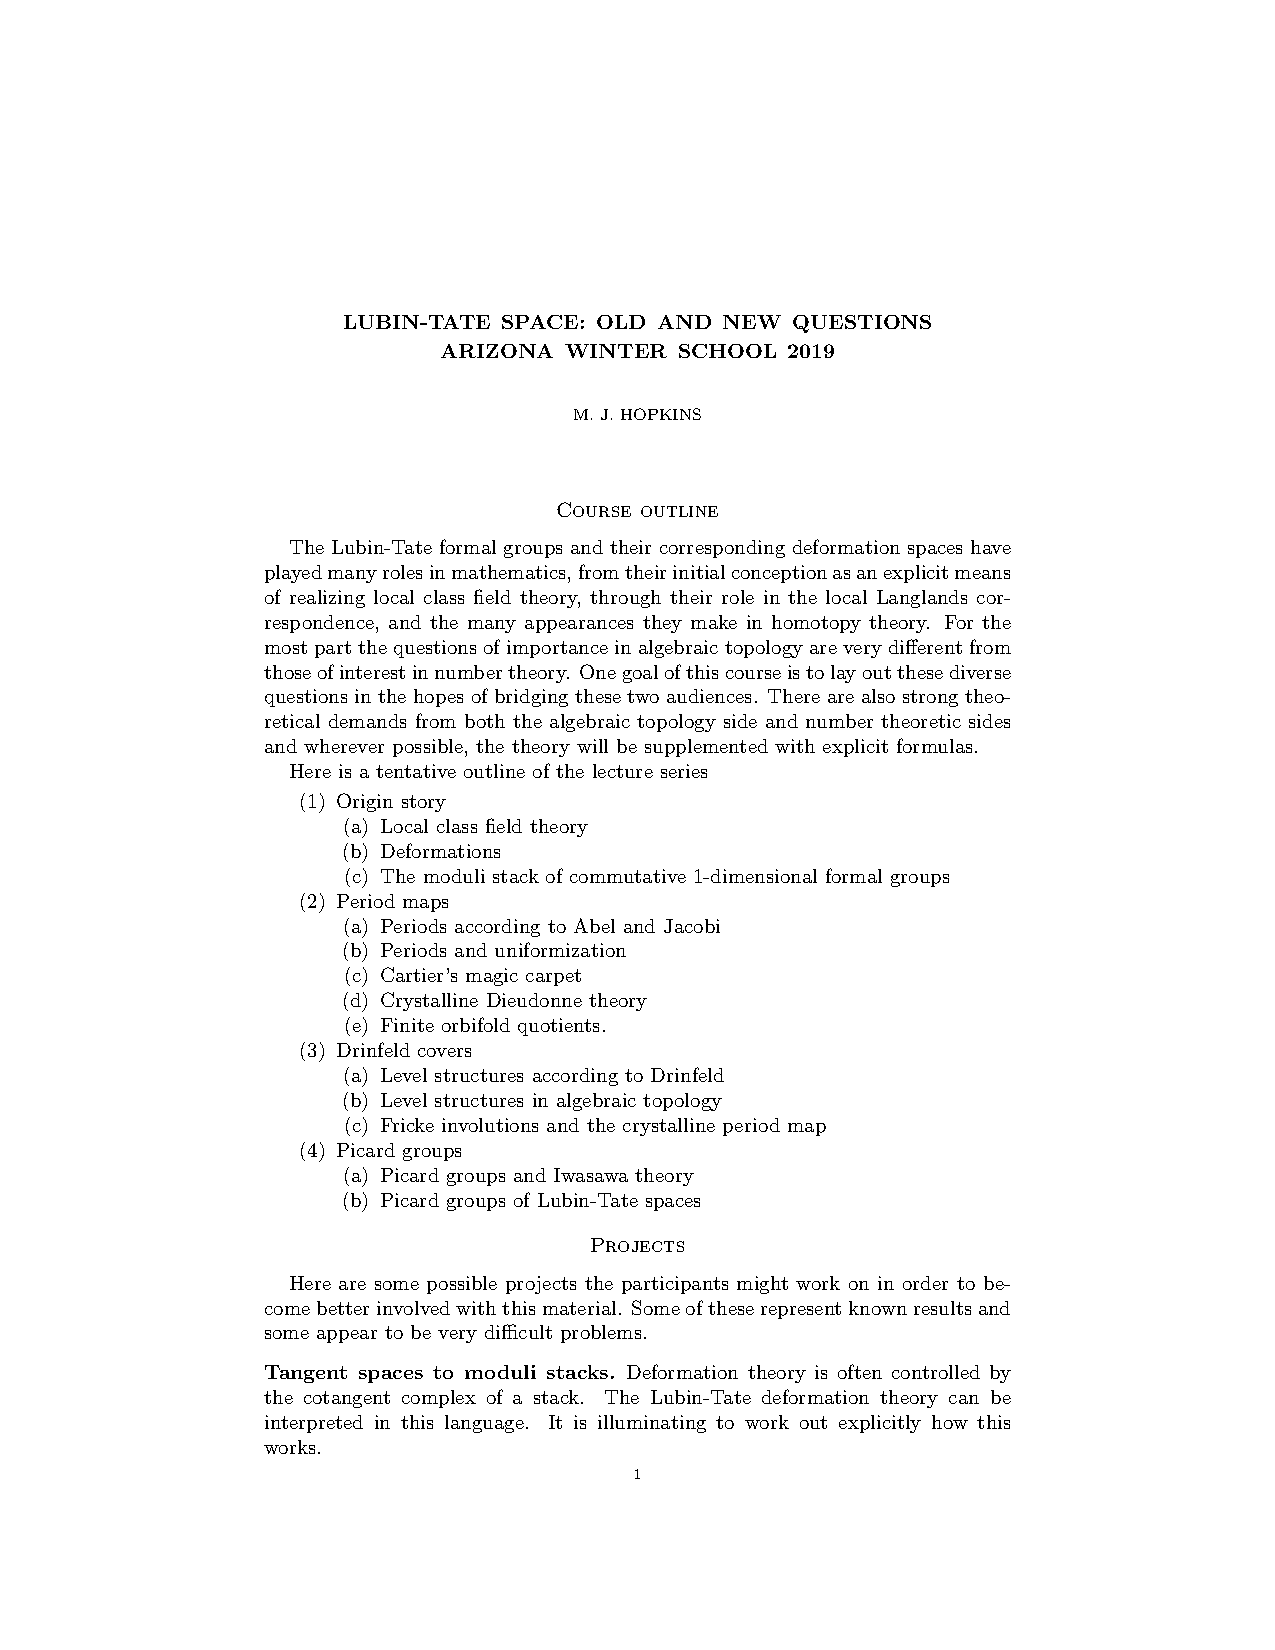
\includepdf[pages=-,scale=1,pagecommand={\thispagestyle{normal}}]{../notes/hopkins/2019HopkinsOutline.pdf}
\phantomsection
\addtocounter{subsection}{1}
\addcontentsline{toc}{subsection}{\protect\numberline{\thesubsection} Lecture Notes \& Project Description}
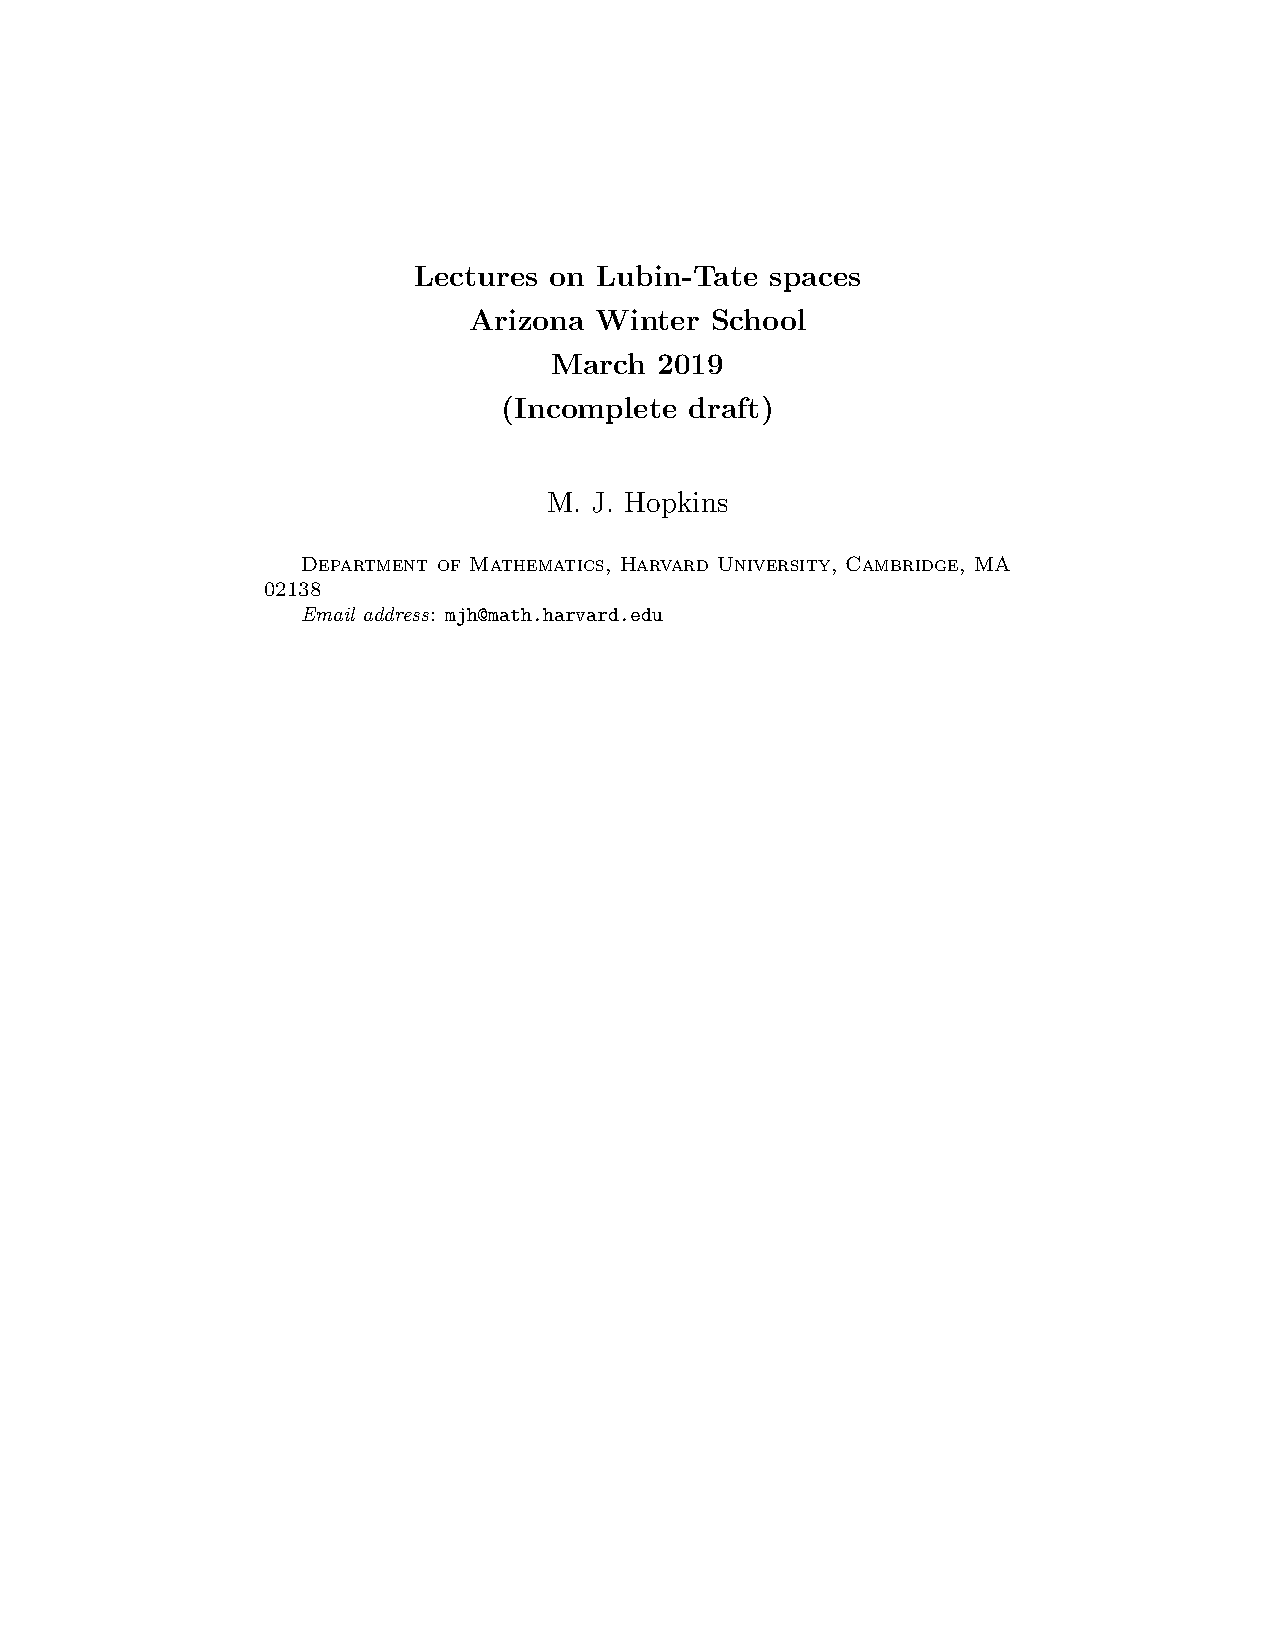
\includepdf[pages=-,scale=1,pagecommand={\thispagestyle{normal}}]{../notes/hopkins/2019HopkinsNotes.pdf}

% Lurie
\phantomsection
\addtocounter{section}{1}
\addcontentsline{toc}{section}{\protect\numberline{\thesection} Jacob Lurie: Tamagawa numbers in the function field case}
\phantomsection
\setcounter{subsection}{1}
\addcontentsline{toc}{subsection}{\protect\numberline{\thesubsection} Course \& Project Outline}
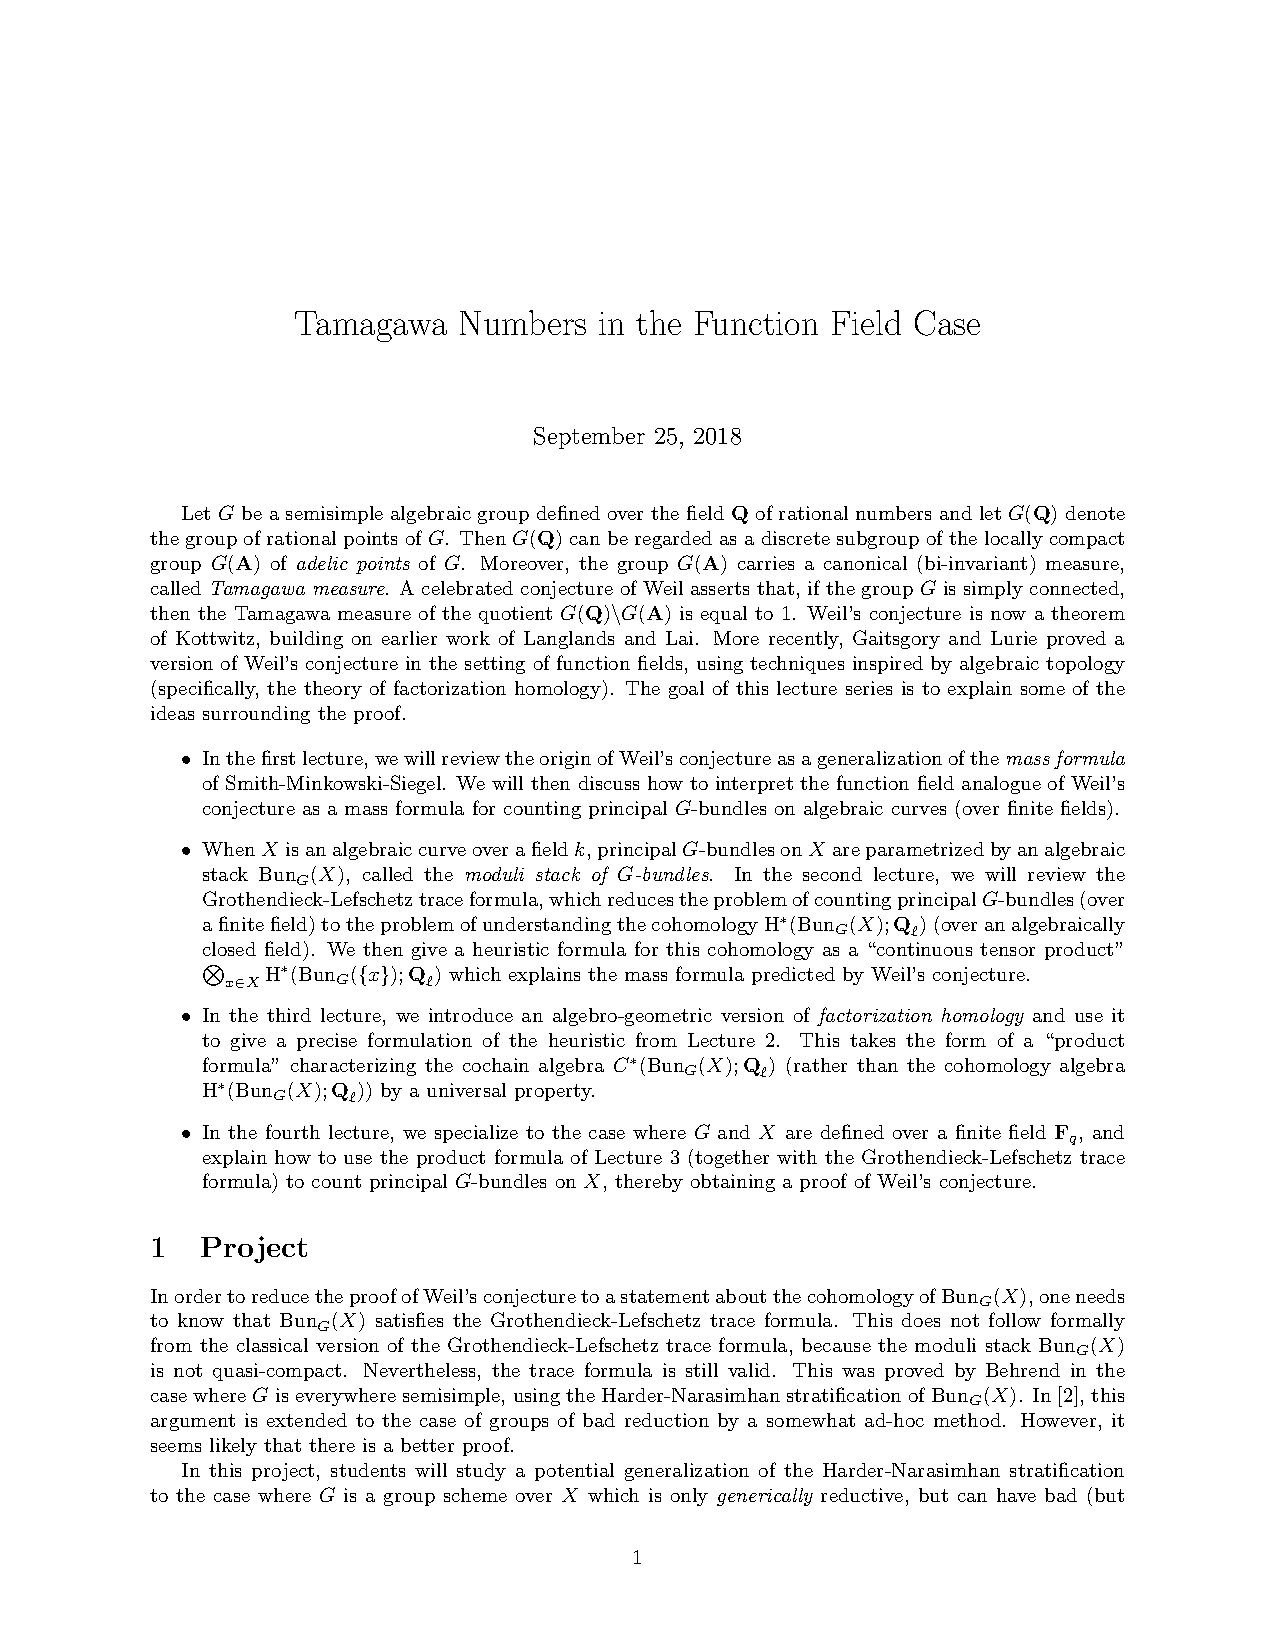
\includepdf[pages=-,scale=1,pagecommand={\thispagestyle{normal}}]{../notes/lurie/2019LurieOutline.pdf}
\phantomsection
\addtocounter{subsection}{1}
\addcontentsline{toc}{subsection}{\protect\numberline{\thesubsection} Lecture Notes \& Project Description}
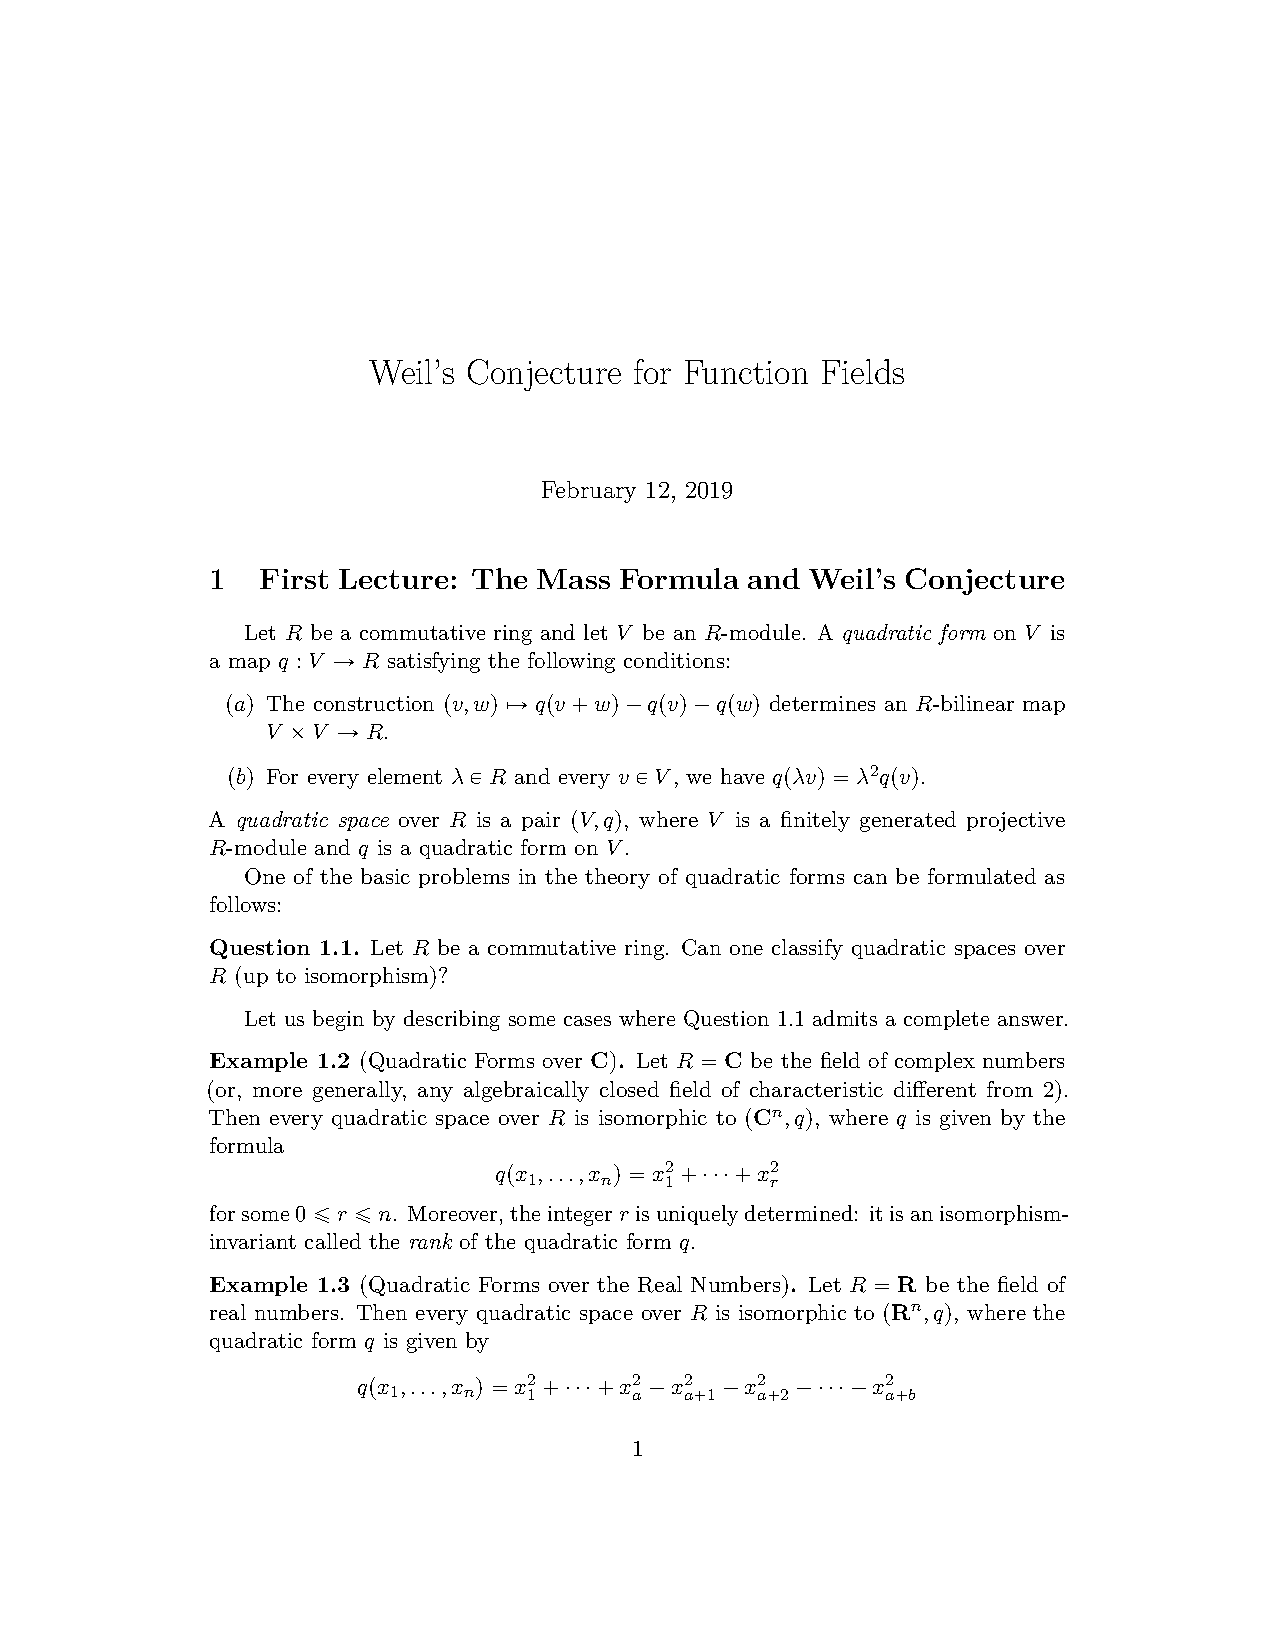
\includepdf[pages=-,scale=1,pagecommand={\thispagestyle{normal}}]{../notes/lurie/2019LurieNotes.pdf}

% Morrow
\phantomsection
\addtocounter{section}{1}
\addcontentsline{toc}{section}{\protect\numberline{\thesection} Matthew Morrow: Topological Hochschild homology in arithmetic geometry}
\phantomsection
\setcounter{subsection}{1}
\addcontentsline{toc}{subsection}{\protect\numberline{\thesubsection} Course \& Project Outline}
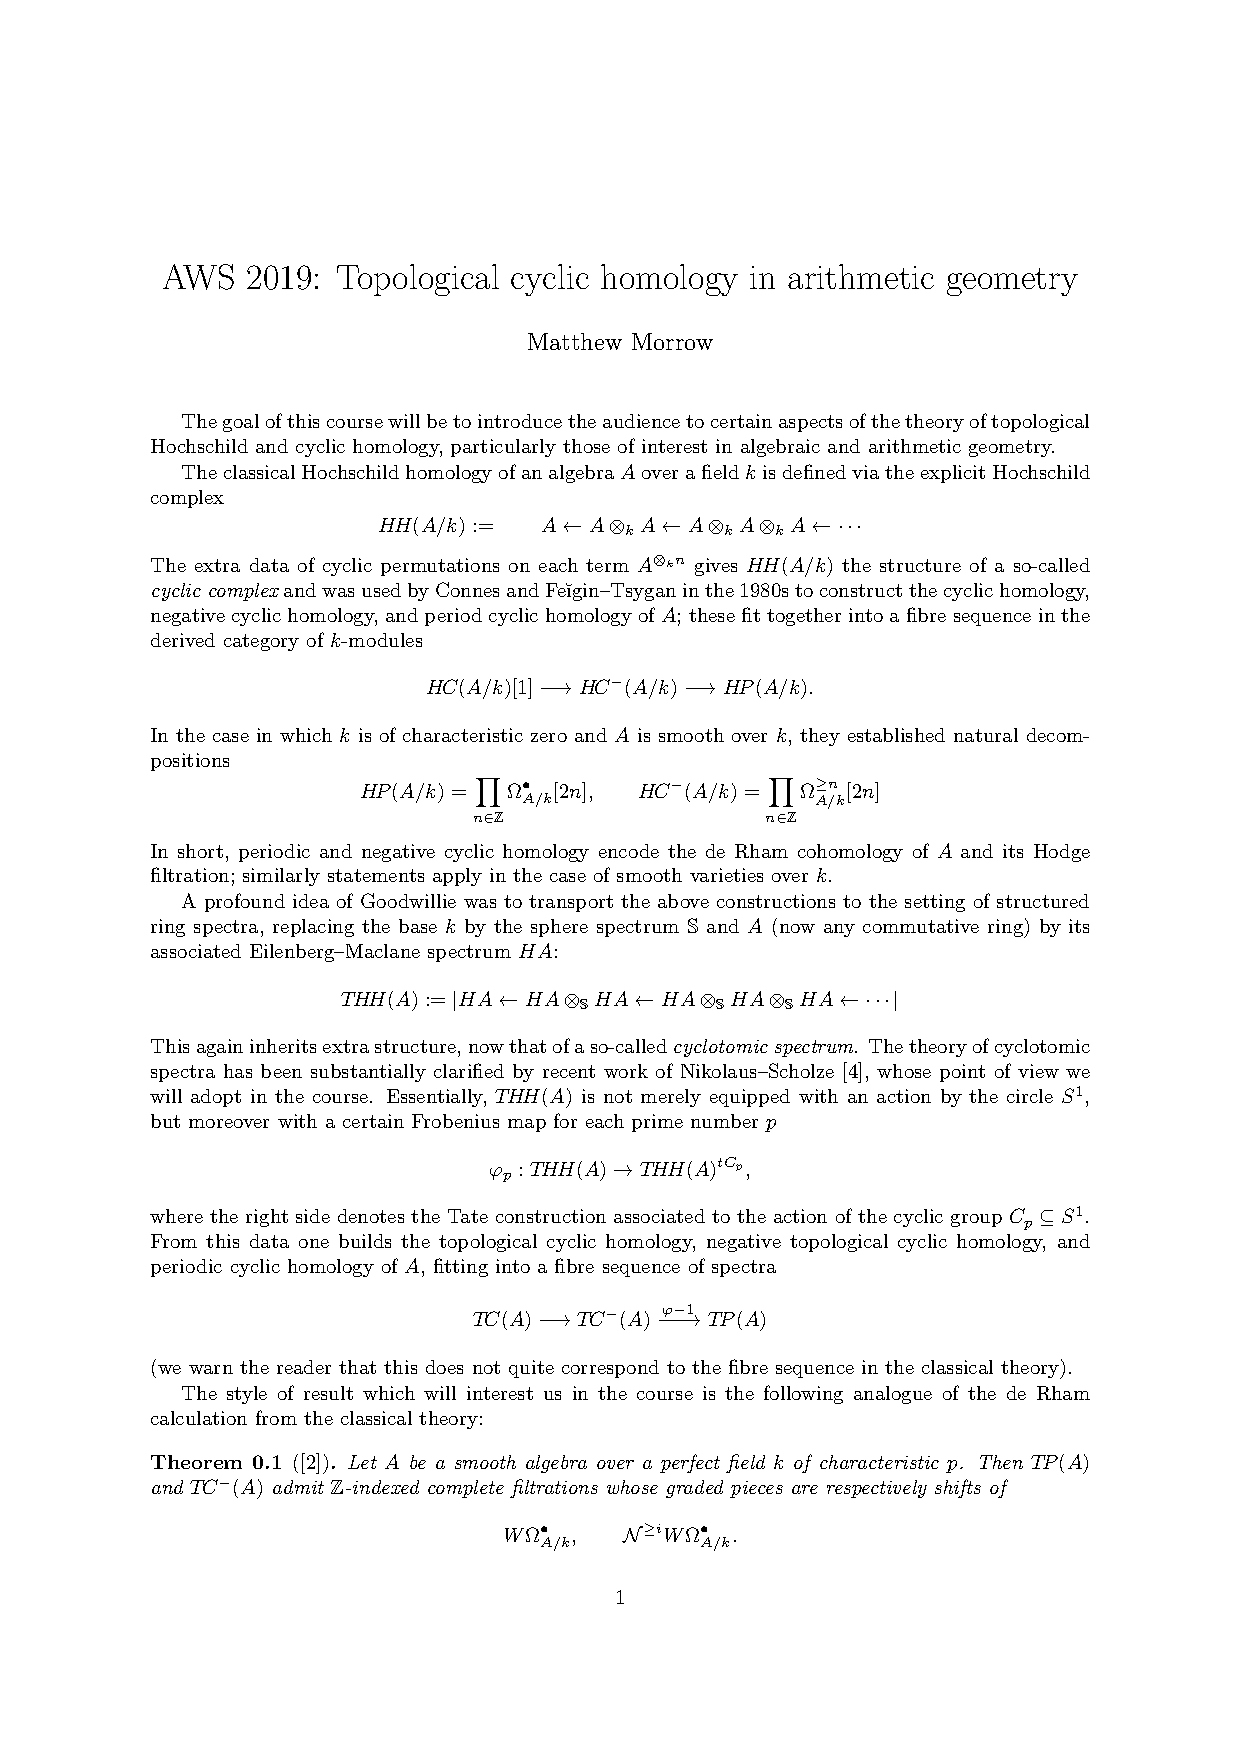
\includepdf[pages=-,scale=1,pagecommand={\thispagestyle{normal}}]{../notes/morrow/2019MorrowOutline.pdf}
\phantomsection
\addtocounter{subsection}{1}
\addcontentsline{toc}{subsection}{\protect\numberline{\thesubsection} Lecture Notes \& Project Description}
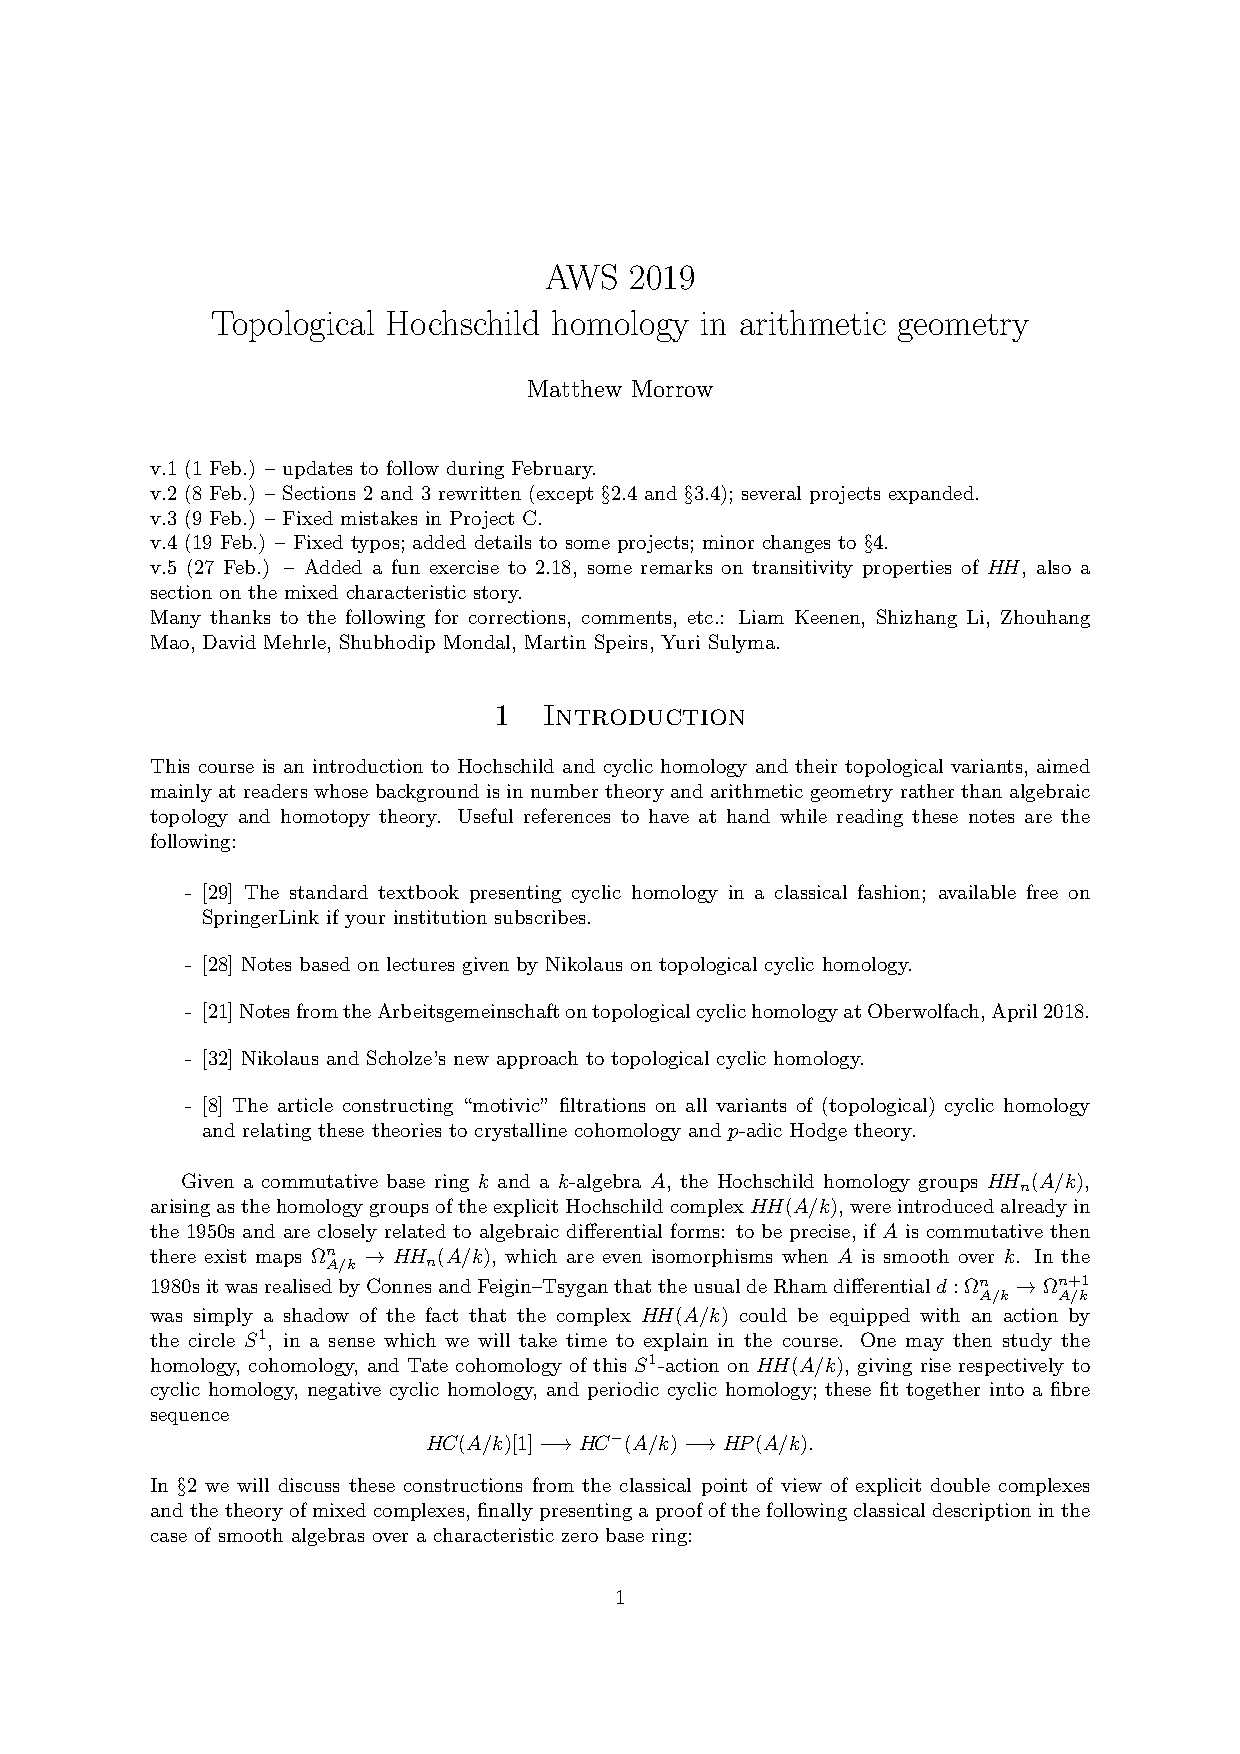
\includepdf[pages=-,scale=1,pagecommand={\thispagestyle{normal}}]{../notes/morrow/2019MorrowNotes.pdf}

% Wickelgren
\phantomsection
\addtocounter{section}{1}
\addcontentsline{toc}{section}{\protect\numberline{\thesection} Kirsten Wickelgren: $\A^1$-enumerative geometry}
\phantomsection
\setcounter{subsection}{1}
\addcontentsline{toc}{subsection}{\protect\numberline{\thesubsection} Course \& Project Outline}
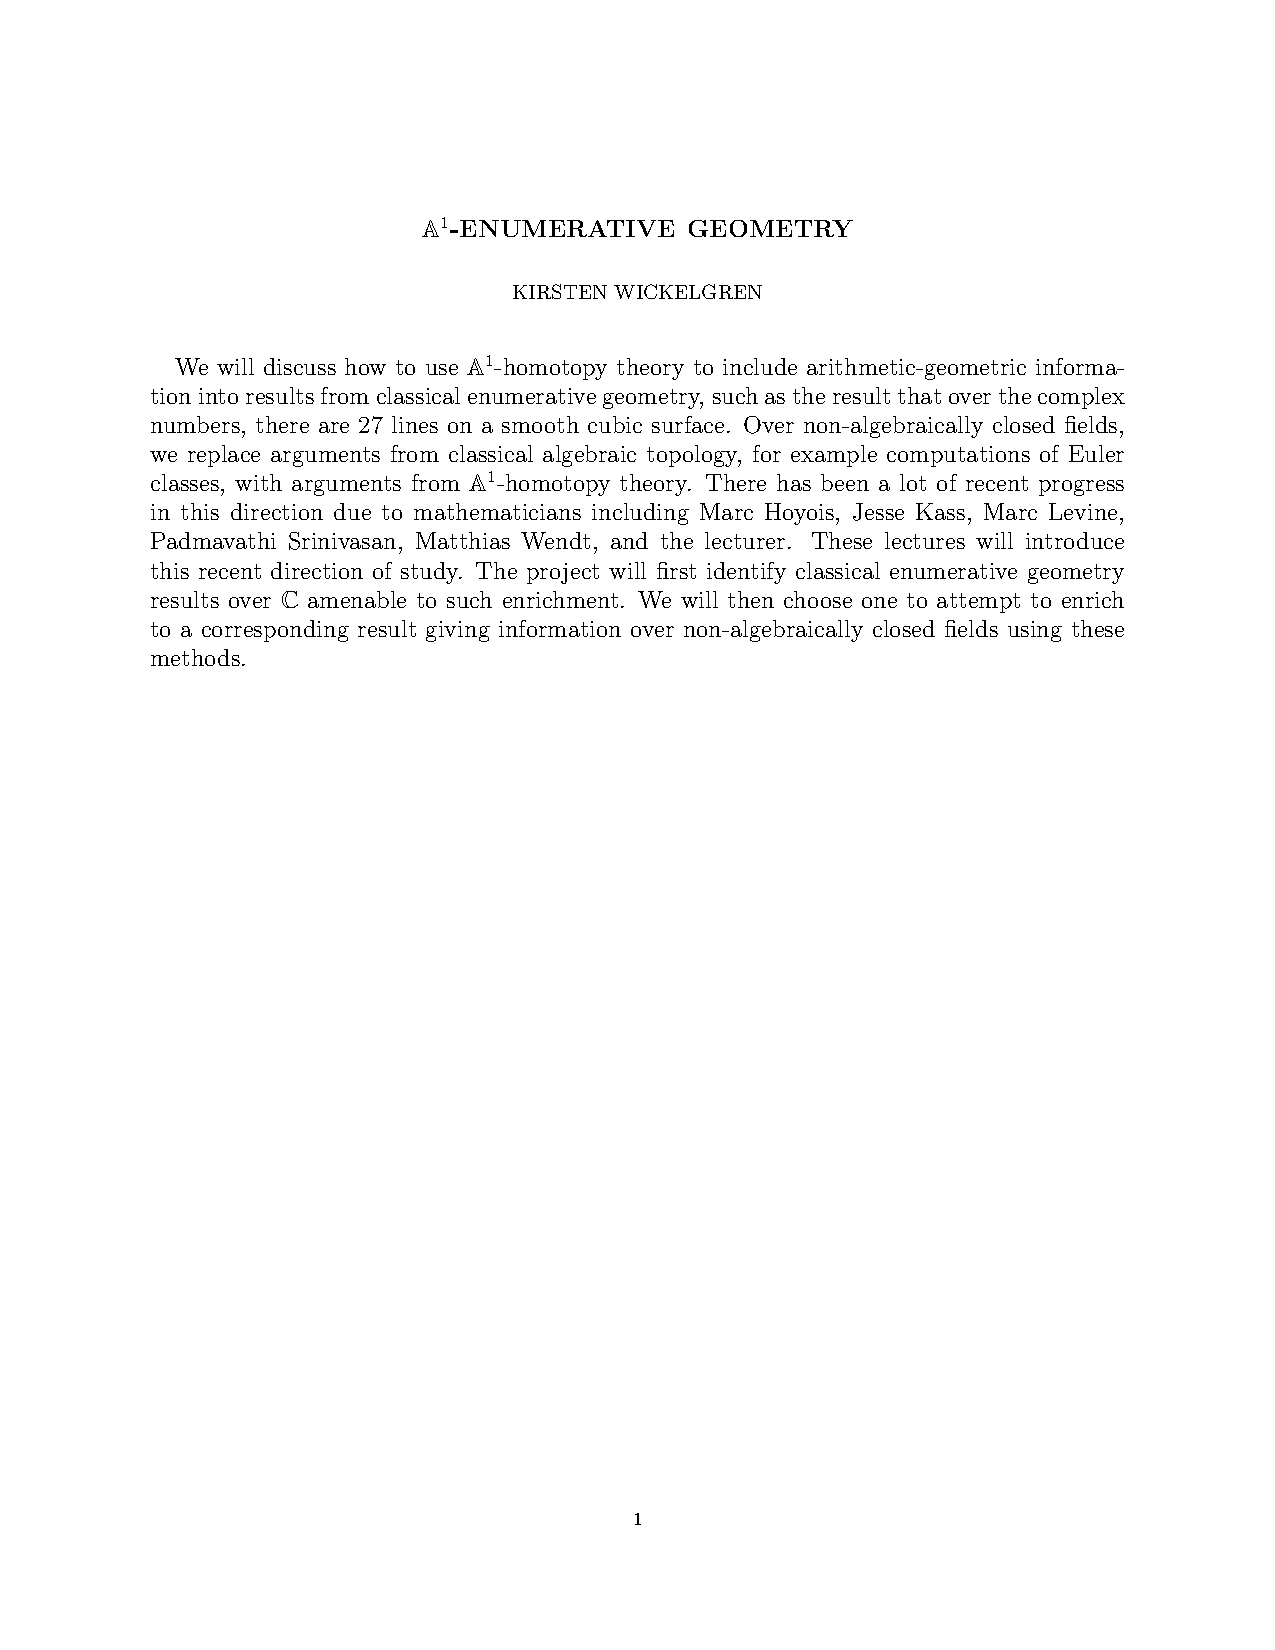
\includepdf[pages=-,scale=1,pagecommand={\thispagestyle{normal}}]{../notes/wickelgren/2019WickelgrenOutline.pdf}
\phantomsection
\addtocounter{subsection}{1}
\addcontentsline{toc}{subsection}{\protect\numberline{\thesubsection} Lecture Notes \& Project Description}
\includepdf[pages=-,scale=1,pagecommand={\thispagestyle{normal}}]{../notes/wickelgren/2019WickelgrenNotes.pdf}

% Problem Groups
\phantomsection
\addtocounter{section}{1}
\addcontentsline{toc}{section}{\protect\numberline{\thesection} Problem Sessions}
\phantomsection
\setcounter{subsection}{1}
\addcontentsline{toc}{subsection}{\protect\numberline{\thesubsection} Vesna Stojanoska: Formal groups and cohomology theories}
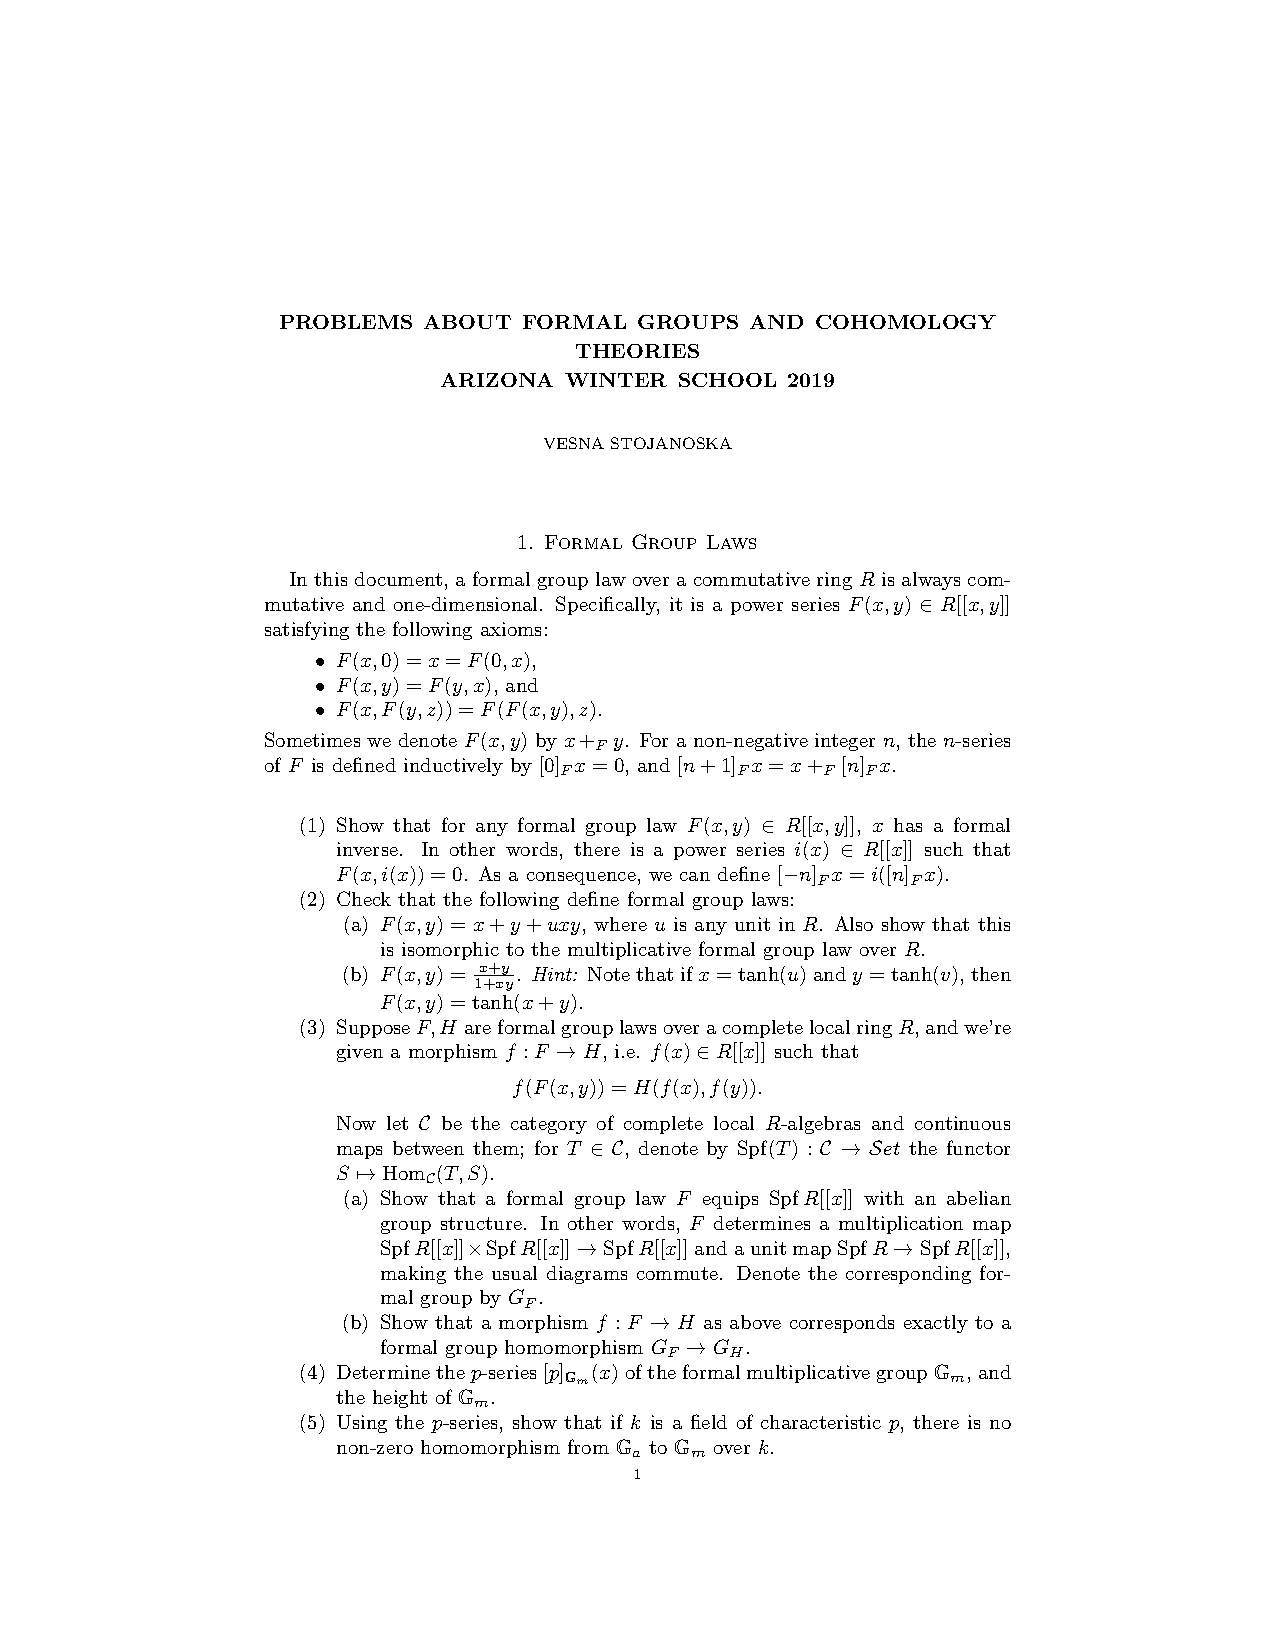
\includepdf[pages=-,scale=1,pagecommand={\thispagestyle{normal}}]{../notes/problem_groups/2019StojanoskaProblems.pdf}
\phantomsection
\addtocounter{subsection}{1}
\addcontentsline{toc}{subsection}{\protect\numberline{\thesubsection} Inna Zakharevich: The geometry of algebra and the algebra of geometry: model categories, infinity categories and spectra}
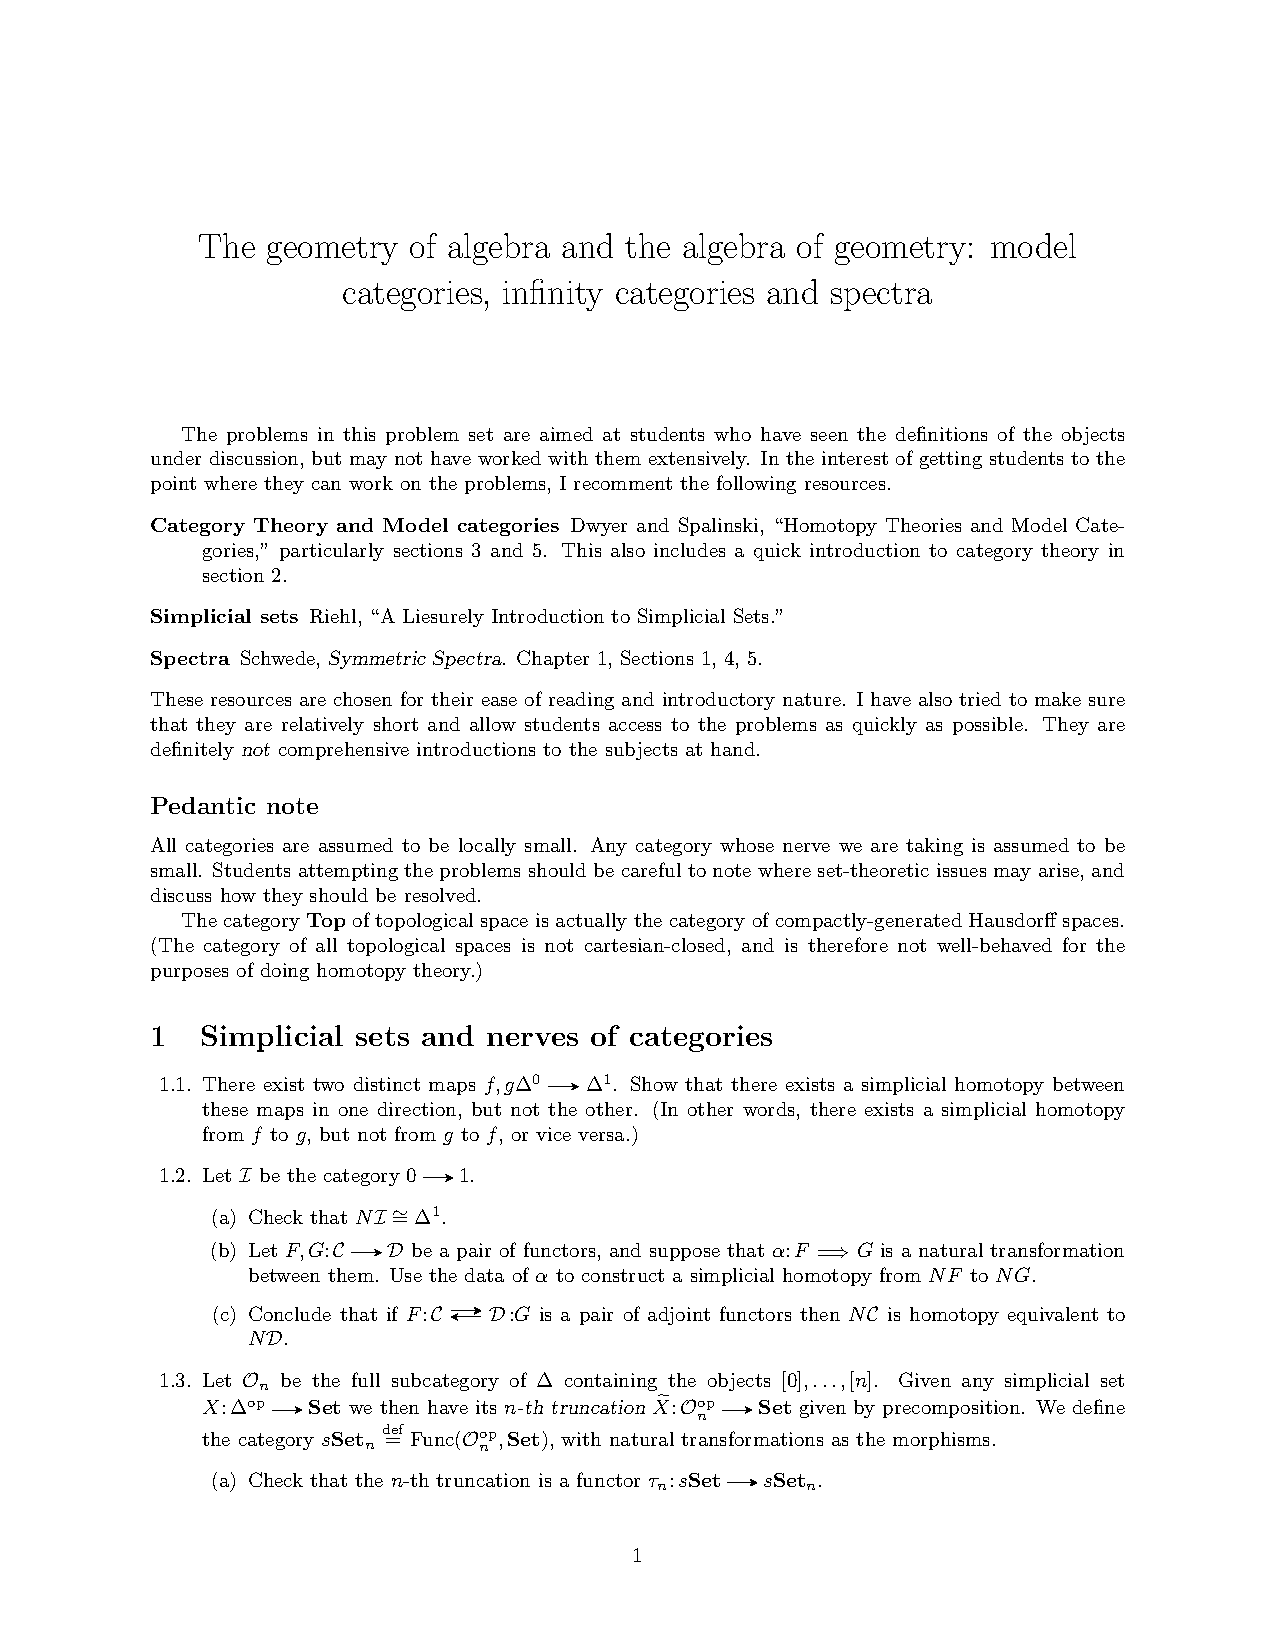
\includepdf[pages=-,scale=1,pagecommand={\thispagestyle{normal}}]{../notes/problem_groups/2019ZakharevichProblems.pdf}
\phantomsection
\addtocounter{subsection}{1}
\addcontentsline{toc}{subsection}{\protect\numberline{\thesubsection} Emily Riehl: A leisurely introduction to simplicial sets}
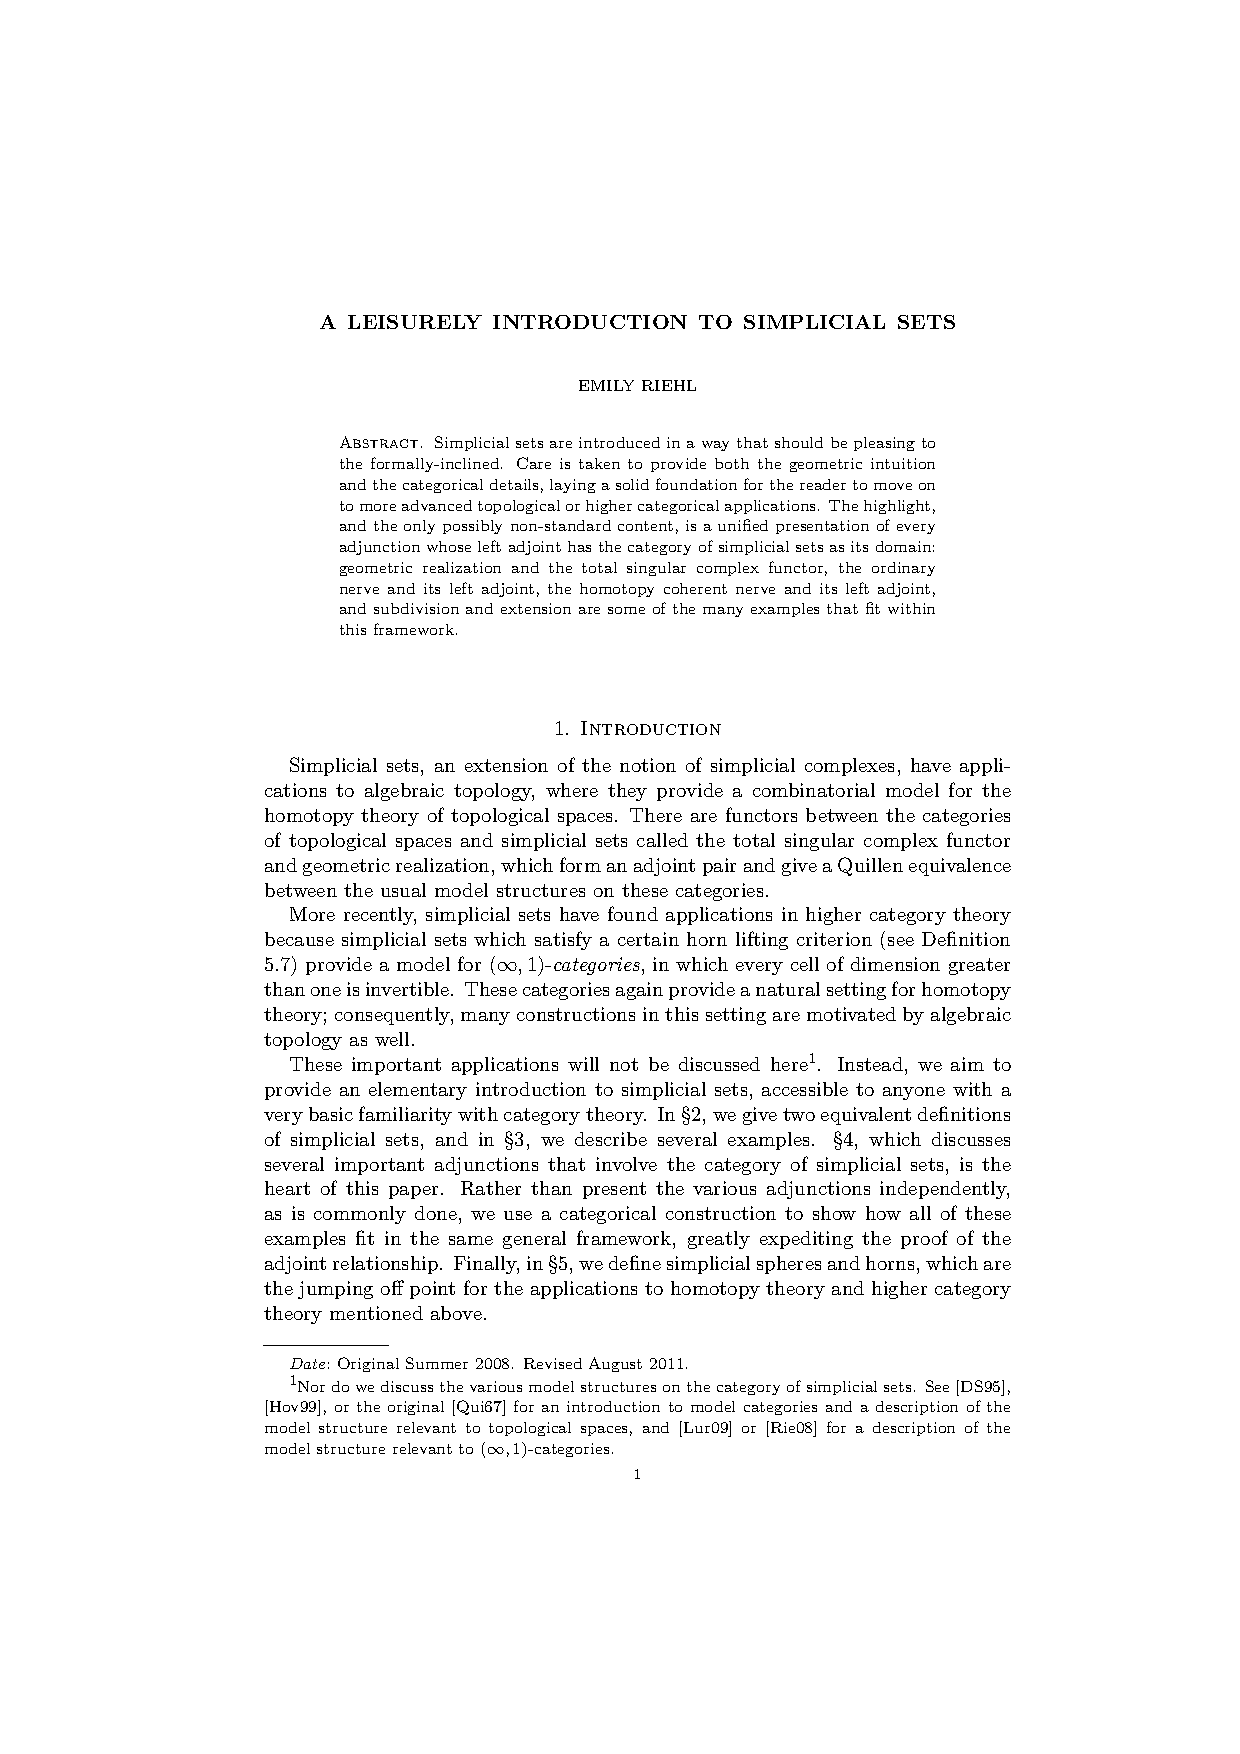
\includepdf[pages=-,scale=1,pagecommand={\thispagestyle{normal}}]{../notes/problem_groups/ssets.pdf}
\phantomsection
\addtocounter{subsection}{1}
\addcontentsline{toc}{subsection}{\protect\numberline{\thesubsection} Martin Speirs: Formal groups and cohomology theories reading projects for Morrow study group}
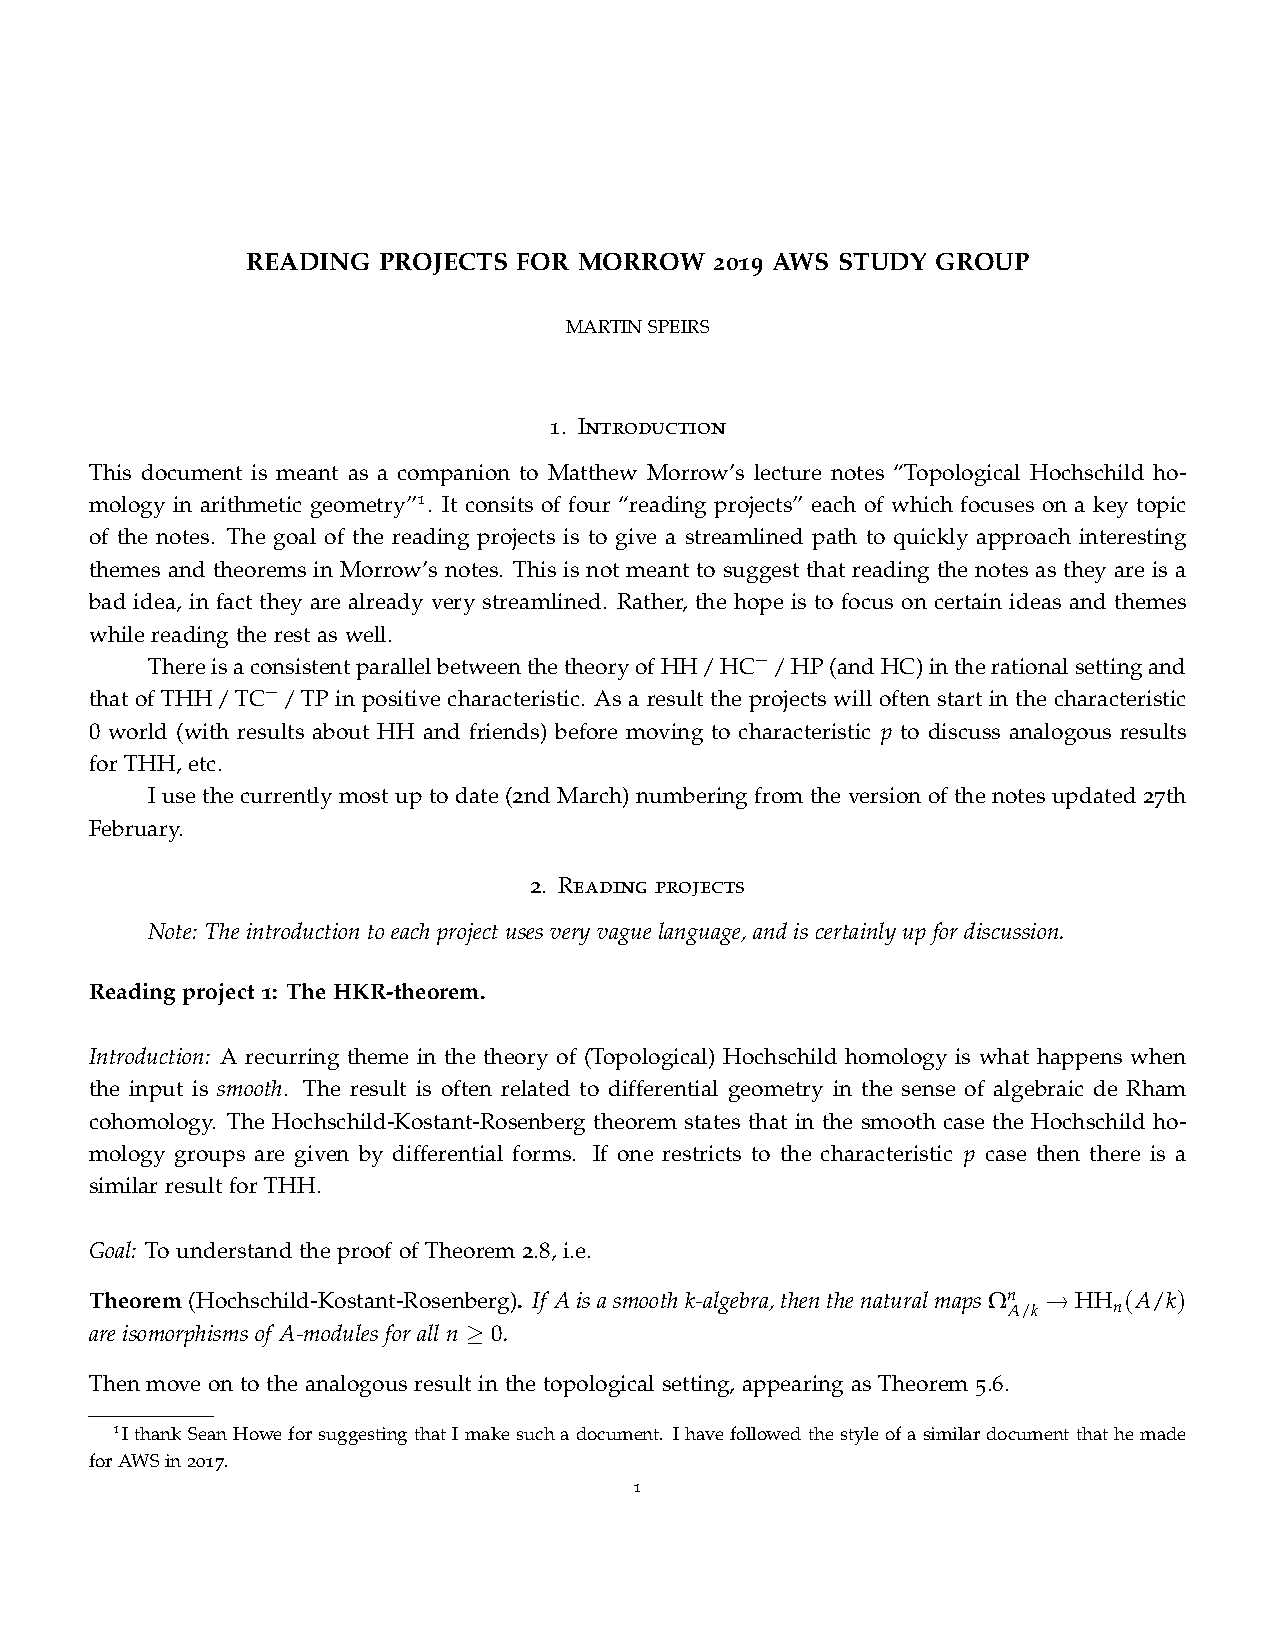
\includepdf[pages=-,scale=1,pagecommand={\thispagestyle{normal}}]{../notes/problem_groups/2019SpeirsStudyNotes.pdf}
}


% -------------------
% Bibliography
% -------------------
\newpage
\nocite{*}
\printbibliography

\end{document}